%                                                                 aa.dem
% AA vers. 9.1, LaTeX class for Astronomy & Astrophysics
% demonstration file
%                                                       (c) EDP Sciences
%-----------------------------------------------------------------------
%
%\documentclass[referee]{aa} % for a referee version
%\documentclass[onecolumn]{aa} % for a paper on 1 column  
%\documentclass[longauth]{aa} % for the long lists of affiliations 
%\documentclass[letter]{aa} % for the letters 
%\documentclass[bibyear]{aa} % if the references are not structured 
%                              according to the author-year natbib style

%
\documentclass{aa}  

%
\usepackage{graphicx}
%%%%%%%%%%%%%%%%%%%%%%%%%%%%%%%%%%%%%%%%
\usepackage{txfonts}
\usepackage{amsmath}
\usepackage{amssymb}
\usepackage{booktabs}
\usepackage{subcaption}
\usepackage{gensymb}
\usepackage{placeins}
%%%%%%%%%%%%%%%%%%%%%%%%%%%%%%%%%%%%%%%%
\usepackage[breaklinks=true,colorlinks=true,citecolor=blue,linkcolor=blue,urlcolor=blue]{hyperref}
% To add links in your PDF file, use the package "hyperref"
% with options according to your LaTeX or PDFLaTeX drivers.
%
\begin{document} 

   \title{Deep Learning for Lunar Surface Feature Recognition:
          A Comparative Study of Segmentation and Detection Architectures}

   \author{G. Venturato\inst{1}
          \and
          A. Rahpeyma\inst{1}
          \and
          A.~M. Saiedi Saber\inst{1}
          \and
          G. Vagnoni\inst{1}
          }

   \institute{Physics of Data, Department of Physics and Astronomy,
              University of Padova, Via Marzolo 8, I-35131 Padova, Italy}

   \date{Received June 13, 2026; accepted}

   \abstract
   % context heading (optional)
    {Lunar reconnaissance missions generate high-resolution imagery at volumes that make manual geological mapping infeasible, driving the need for automated detection and segmentation of surface features.}
   % aims heading (mandatory)
    {This work compares four approaches to lunar geomorphological feature recognition---a classical thresholding-and-morphology baseline, semantic segmentation (SmallUNet), instance segmentation (Mask R-CNN), and single-stage object detection (YOLOv8)---on the same dataset, the same leakage-free spatial split, and the same metrics, in order to establish which formulation is preferable for which feature class and at what computational cost.}
   % methods heading (mandatory)
    {All methods are trained and evaluated on 15\,931 overlapping tiles of the Marius Hills region carrying seven semantic feature channels. A shared evaluation protocol reduces every method to per-class binary masks on a spatially disjoint validation set, scored with prevalence-robust metrics (Matthews correlation alongside F1/IoU) and per-method calibrated thresholds. Dedicated experiments quantify two methodological hazards of the dataset: the near-saturated impact-crater channel (82\% pixel prevalence) and the train--validation leakage induced by 50\%-overlapping tiles under random splitting.}
   % results heading (mandatory)
    {On the saturated crater channel, F1 and IoU are dominated by the base rate: a trivial predict-everything baseline attains F1 $= 0.90$, and the SmallUNet reproduces it with MCC $\approx 0$ in every regime. Read on the skill metric, the best crater method flips with the regime: on crater-sparse tiles Mask R-CNN leads (MCC 0.19) ahead of YOLOv8 (0.16), on dense tiles only YOLOv8 keeps a positive signal (0.24). On wrinkle ridges---the class with genuine supervision---the ranking reverses: SmallUNet is best (MCC 0.45) ahead of Mask R-CNN (0.37), with YOLOv8 (0.08) and a classical Sato-filter baseline ($\approx 0$) far behind, at 1/60th of Mask R-CNN's inference cost. Identical YOLOv8 detectors retrained under a random tile split versus the spatial split quantify the protocol's impact on reported scores.}
   % conclusions heading (optional), leave it empty if necessary
     {The preferable architecture depends on the class regime: semantic segmentation wins where dense pixel supervision exists, instance detection wins for sparse countable objects, and no architecture can rescue a channel without genuine supervision. Evaluation-protocol choices (split geometry, metric, threshold) shift reported scores by more than any architectural choice studied here, and must be fixed before architectures are compared.}

    \keywords{Moon -- lunar surface features -- deep learning -- instance segmentation -- semantic segmentation -- object detection}

   \titlerunning{Deep Learning for Lunar Surface Feature Recognition}
   \authorrunning{Venturato et al.}

   \maketitle


%-------------------------------------------------------------------

\section{Introduction}
\label{sec:introduction}

High-resolution orbital imagery from the Lunar Reconnaissance Orbiter (LRO) now covers the Moon at resolutions down to half a metre per pixel, far beyond manual analysis capacity \citep{lroc_usgs}. Impact craters, wrinkle ridges, lobate scarps, and lava-tube skylights encode the thermal, tectonic, and impact history of the lunar surface, and their automated identification is a prerequisite for geological mapping and the selection of future landing sites \citep{pia12954,nasa2023southpole}. The computer-vision literature offers several distinct formulations of this task --- semantic segmentation (a label per pixel), instance segmentation (individual objects with masks), single-stage object detection (bounding boxes), and classical image processing --- and it is not obvious a priori which suits planetary terrain: published comparisons are typically confounded by differences in datasets, train/test splits, metrics, and operating thresholds.

This work removes those confounds by comparing one representative of each family --- a thresholding-and-morphology baseline, a compact U-Net (SmallUNet), an adapted Mask R-CNN, and YOLOv8 --- on the \emph{same} data, the \emph{same} leakage-free spatial split, and the \emph{same} metrics. The comparison is organised per feature class rather than per architecture, because the label channels range from an impact-crater layer covering 82\% of all pixels to classes with fewer than one positive pixel in $10^{4}$, and no single aggregate ranking is meaningful across that range. Two methodological experiments frame it. First, we show that the saturated crater channel reduces naive scores to a base-rate artefact --- a predict-everything baseline attains F1 $=0.90$ --- and adopt prevalence-robust metrics accordingly. Second, we quantify the train--validation leakage induced by 50\%-overlapping tiles, by retraining identical detectors under a random tile split and under a spatial block split. Sections~\ref{sec:classical}--\ref{sec:yolo} document the four methods; Sect.~\ref{sec:comparison} presents the shared-protocol comparison and the split-protocol study; Sect.~\ref{sec:southpole} deploys the pipelines on the unlabelled lunar south pole as a transfer diagnostic. The central methodological finding is that on planetary datasets with extreme prevalence structure, the evaluation protocol --- split geometry, metric choice, threshold calibration --- moves reported numbers by more than any architectural decision we tested, and must be fixed before architectures are compared.


\section{Data and shared evaluation protocol}
\label{sec:mr_dataset}

\paragraph{Dataset.}
Training data are Wide Angle Camera (WAC) grayscale tiles from the LROC archive covering the \textit{Marius Hills} volcanic region \citep{mariusdata}, a site of particular interest for its high density of pit skylights, wrinkle ridges, and rilles. The raster is divided by a sliding window into $256\times256$ tiles with stride 128 (50\% overlap between neighbours); tiles without labelled features are kept with probability $p=0.1$, giving 15{,}931 tiles in total. Each tile carries seven binary semantic mask channels --- \texttt{impact\_crater}, \texttt{pit\_skylight}, \texttt{wrinkle\_ridge}, \texttt{lobate\_scarp}, \texttt{irregular\_mare\_patch}, \texttt{apollo\_site}, \texttt{candidate\_rille} --- rasterised from the LROC feature catalogue, with a small per-class morphological dilation for point- and line-like classes (disk radius 2--5\,px; none for craters, which are already area features). Because multiple classes can coexist in a single pixel (e.g.\ a pit on the rim of a crater), the labels are independent binary channels rather than a single-label partition; the segmentation networks consume the pixel masks directly, while the detection methods convert connected components into object instances (Sects.~\ref{sec:maskrcnn} and~\ref{sec:yolo}).

\paragraph{Label prevalence and channel saturation.}
Table~\ref{tab:prevalence} reports the fraction of positive pixels per class over all tiles. The imbalance is extreme \emph{in both directions}: the \texttt{impact\_crater} channel covers 82.1\% of all pixels --- and in 50.7\% of the tiles \emph{every} pixel is positive --- while the five rarest classes have prevalences below $1.4\times10^{-4}$. The crater channel therefore behaves closer to a coverage-like layer than to a sparse target feature. This has a direct consequence for interpretation: the Average Precision (AP) of an uninformative predictor equals the class prevalence, so per-class AP must be read against the baselines in Table~\ref{tab:prevalence} rather than against zero. This single property of the labels shapes the entire comparison of Sect.~\ref{sec:comparison}.

\begin{table}[htbp]
\centering
\caption{Per-class positive-pixel prevalence over the full dataset (15{,}931 tiles, $1.04\times10^9$ pixels per channel). The prevalence is also the AP of an uninformative (chance-level) predictor for that class.}
\label{tab:prevalence}
\resizebox{\columnwidth}{!}{%
\begin{tabular}{lrr}
\toprule
Class & Prevalence & Tiles fully covered \\
\midrule
\texttt{impact\_crater}        & $8.21\times10^{-1}$ & 50.7\% \\
\texttt{wrinkle\_ridge}        & $6.38\times10^{-3}$ & 0 \\
\texttt{lobate\_scarp}         & $1.34\times10^{-4}$ & 0 \\
\texttt{pit\_skylight}         & $4.2\times10^{-5}$  & 0 \\
\texttt{irregular\_mare\_patch} & $2.0\times10^{-5}$  & 0 \\
\texttt{apollo\_site}          & $1.5\times10^{-5}$  & 0 \\
\texttt{candidate\_rille}      & $1.0\times10^{-5}$  & 0 \\
\bottomrule
\end{tabular}
}
\end{table}

\subsection{Train/validation splitting: the leakage problem}
\label{sec:splits}

Because adjacent tiles overlap by 50\%, splitting \emph{tiles} at random does not split \emph{pixels}: a direct measurement on the tile index shows that every validation tile of a random 80/20 split overlaps at least one training tile. Validation scores obtained this way partially reward memorisation of pixels seen during training. Two protocols therefore appear in this paper, and every table states which one it uses: the \textbf{random tile split} (80/20, fixed seed), used by the historical single-method experiments --- comparisons \emph{within} it, between configurations trained on the identical split, remain internally valid, but absolute scores are optimistic --- and the \textbf{spatial block split} (the reference protocol), in which contiguous 1024-px spatial blocks are assigned to validation and every training tile whose footprint intersects a validation tile is discarded, so train and validation are strictly disjoint in pixel space (11{,}289 train / 3{,}248 validation tiles, 1{,}394 boundary tiles dropped, zero pixel overlap, verified by an independent assertion). All cross-method numbers in Sect.~\ref{sec:comparison} use the spatial split with seed 42; Sect.~\ref{sec:split_study} quantifies the difference between the protocols directly.

\subsection{Shared metrics}
\label{sec:metrics_protocol}

For the cross-method comparison every model is reduced to the same output format --- a per-class binary mask on each validation tile --- so that segmentation networks, detectors (boxes filled as mask regions), and the classical baseline are scored identically. Per class we report pixel precision, recall, F1, and IoU at a per-method operating threshold $\tau$ calibrated on a held-out subset of the validation split (no method is penalised by a foreign operating point); the \textbf{Matthews correlation coefficient (MCC)} as the primary ranking metric --- unlike F1 and IoU it is invariant to the positive-class base rate: on the 82\%-prevalence crater channel a predict-everything baseline attains F1 $=0.90$ and IoU $=0.82$ but MCC $=0$ by construction; object count error (mean absolute error of connected-component counts) as an instance-level diagnostic; and inference cost in ms per tile on identical hardware. For threshold-free evaluation of the segmentation networks we additionally report AP, always against the prevalence baselines of Table~\ref{tab:prevalence}. The lunar south pole tiles of Sect.~\ref{sec:southpole} have no feature catalogue and hence no ground truth; south-pole outputs are treated as transfer \emph{diagnostics} (prediction-confidence statistics), never as accuracy metrics.


\section{Classical baseline: thresholding and morphology}
\label{sec:classical}

Before any learned method, we establish what classical image processing achieves on the same protocol: a deep model is only interesting if it beats interpretable, millisecond-scale processing. The \emph{crater detector} exploits the fact that craters appear as locally dark depressions under the fixed WAC illumination: each tile is normalised, adaptive (local-mean) thresholding isolates dark regions, and morphological opening/closing plus a minimum-area filter clean the result into a binary crater mask. The pipeline has five interpretable parameters (threshold offset, window size, two kernel radii, minimum area), tuned on the calibration subset of the spatial validation split only. Wrinkle ridges are curvilinear, so the \emph{ridge detector} instead uses the Sato vesselness filter (Hessian eigenvalues at multiple scales), which responds to elongated bright structures, followed by the same morphological cleaning and threshold calibration.

The baseline runs at ${\sim}1$\,ms per tile on a single CPU core --- three orders of magnitude cheaper than Mask R-CNN --- and every decision it makes can be inspected. Its scores in Sect.~\ref{sec:comparison} define the floor that justifies (or fails to justify) the learned methods class by class.


\section{Instance segmentation with a custom Mask R-CNN}
\label{sec:maskrcnn}

The first learned formulation treats lunar features as \emph{instances}: for every tile, a list of individual feature objects, each with its own class label, bounding box, and pixel-level mask. Mask R-CNN \citep{he2017maskrcnn} is the natural tool, because it predicts a segmentation mask in parallel with the detection of each object.

\paragraph{Instance-target preparation.}
A semantic channel is not the same thing as a set of objects. Before training, every channel is audited: only channels labelled in at least 200 tiles are kept, and channels whose mean coverage exceeds 20\% of the tile are flagged as coverage-like rather than object-like. Training therefore uses four classes: impact crater, pit/skylight, wrinkle ridge, and lobate scarp. Each selected channel is converted into instances by connected-component labelling (8-connectivity); components smaller than 30\,px or larger than 6000\,px are discarded, slivers narrower than 3\,px are dropped, and instances are capped at 100 per tile. This step is deliberately conservative, because noisy targets propagate directly into poor detections. A spatial band (the right-most tile columns) is held out for validation, and training tiles are augmented with geometric transforms plus brightness/contrast jitter.

\paragraph{Architecture and training.}
The backbone is a COCO-pretrained ResNet-50 with a Feature Pyramid Network \citep{he2016resnet,lin2017fpn}, lowest layers frozen and the top three trainable. Three changes adapt it to lunar tiles: anchors retuned to lunar scales (one size per FPN level, $(8,16,32,64,128)$\,px, aspect ratios $(0.5,1,2)$, preserving the pretrained RPN head shape); a deeper four-layer box head (1024 units, dropout 0.10); and a residual convolutional mask head (four residual blocks, 256 channels, GroupNorm) with transposed-convolution upsampling; the final model totals 50.8M parameters. The native 256\,px resolution is kept instead of torchvision's 800\,px rescaling. Optimisation uses AdamW \citep{loshchilov2019adamw} with discriminative learning rates (backbone and RPN at one tenth of the head rate of $2\times10^{-4}$), weight decay $10^{-4}$, one-epoch warm-up with cosine decay, and gradient clipping at 5.0, for 20 epochs at batch size 8. Because the only available hardware was a CPU (${\sim}$half a day per run), the loop was engineered to be crash-safe and resumable, checkpointing model, optimiser, and scheduler state every epoch.

\paragraph{Results.}
Table~\ref{tab:metrics} collects the validation metrics of the best checkpoint (epoch 8; validation loss turns upward after ${\sim}4$ epochs, indicating overfitting on the limited positives). The two halves of the network tell very different stories. The \emph{segmentation} branch works: whenever a detection is matched to a ground-truth object, the predicted mask overlaps it well (IoU 0.64, Dice 0.77). The \emph{detection} branch is where everything breaks down: mAP@0.5 sits near 1\%, and false negatives (7790) vastly outnumber true positives (461). The per-class breakdown shows that the comparatively common craters and ridges carry essentially all of the average precision, while the scientifically interesting pit/skylight class is barely detected and lobate scarps reach exactly zero --- too few examples to learn from. The training history and qualitative prediction panels are collected in Appendix~\ref{app:maskrcnn}.

\begin{table}[htbp]
\caption{Mask R-CNN validation metrics (best checkpoint, full held-out spatial band), with per-class AP@0.5.}
\label{tab:metrics}
\centering
\small
\begin{tabular}{l r}
\toprule
Metric & Value \\
\midrule
mAP@0.5                       & $0.010$ \\
Precision / Recall / F1       & $0.104$ / $0.056$ / $0.073$ \\
Mean mask IoU / Dice (matched) & $0.636$ / $0.773$ \\
Count MAE (objects per tile)  & $6.30$ \\
True / False pos.\ / False neg.\ & $461$ / $3973$ / $7790$ \\
\midrule
AP@0.5: impact crater          & $0.0233$ \\
\phantom{AP@0.5:} wrinkle ridge   & $0.0172$ \\
\phantom{AP@0.5:} pit / skylight  & $0.0003$ \\
\phantom{AP@0.5:} lobate scarp    & $0.0000$ \\
\bottomrule
\end{tabular}
\end{table}

\paragraph{Lessons.}
Most of what limits the score lies outside the network. Connected-component labelling is a leaky abstraction --- touching craters merge, elongated ridges fragment --- so the supervision is fundamentally noisier than a hand-annotated detection dataset, capping achievable precision. The rarest classes are the scientifically most interesting ones, and frequency-based channel selection cannot manufacture positive examples that are not there. Most instructively, good masks did not buy good detections: mask IoU is measured only on already-matched objects, so the bottleneck is upstream, in proposal recall and classification --- improving the mask head further would not move the headline metric.


\section{Semantic segmentation with a compact U-Net (SmallUNet)}
\label{sec:moon_recognition}

Complementing the instance formulation, the same terrain is addressed as dense, pixel-level labelling: multi-label semantic segmentation, with seven independent binary classifications per pixel (Sect.~\ref{sec:mr_dataset}), posed per class rather than as a single-label softmax problem because classes can coexist in a pixel.

\paragraph{Pre-processing.}
Each grayscale tile is converted into a three-channel tensor providing complementary views of the same image: (i) min-max normalised intensity; (ii) CLAHE (\texttt{skimage} \texttt{equalize\_adapthist}, clip limit 0.03) to enhance local contrast; (iii) the Sobel gradient magnitude, highlighting boundaries and ridge-like structures. Because CLAHE costs ${\sim}3$\,s per tile on CPU, all tensors are precomputed once and cached as compressed \texttt{.npz} files.

\paragraph{Architecture.}
SmallUNet follows the U-Net encoder--decoder paradigm \citep{ronneberger2015unet} at reduced scale: three \emph{Down} blocks ($2\times2$ max-pooling + DoubleConv, i.e.\ two $3\times3$ convolution--BatchNorm--ReLU stages), a symmetric decoder using transposed convolutions and skip-connection concatenation, and a $1\times1$ output head mapping 32 channels to 7 independent logit maps. Two optional components are studied below: residual (ResNet-style) shortcuts inside each DoubleConv block, and spatial Dropout2d at the bottleneck. The base width $w$ scales the channel progression ($w$--$8w$): $w=16/32/64$ gives 0.51M/2.0M/8.0M parameters.

\paragraph{Losses and training.}
Two composite losses are compared: \emph{BCEDice} (binary cross-entropy plus soft Dice, macro-averaged over classes) and \emph{FocalDice}, which replaces BCE with the binary focal loss \citep{lin2017focal} ($\gamma=2$, $\alpha=0.25$) and weights the per-class Dice terms $[1,4,5,5,5,5,5]$ to penalise misdetection of rare classes. Unless noted otherwise, the definitive experiments ran on an NVIDIA Tesla T4 (CloudVeneto) on the full 15{,}931-tile dataset for 30 epochs (batch 16, Adam, cosine annealing $10^{-3}\!\to\!10^{-5}$); local Apple-Silicon runs served for prototyping. Validation is computed every epoch: per-class precision, recall, F1, IoU at $\tau=0.5$, plus threshold-free AP.

\subsection{Ablation campaign}
\label{sec:mr_augmentation}

Three controlled studies were run in sequence; Table~\ref{tab:final_summary} collects the best result of each, and Appendix~\ref{app:unet} the architecture details, loss definitions, full per-study tables, and validation curves.

\paragraph{Study 1 --- architecture.}
Five cumulative configurations (BCEDice; FocalDice; +residual; +dropout $p=0.3$; +both) were compared on the full T4 protocol. Residual shortcuts consistently improve aggregate F1, IoU, and AP; dropout alone does not help, likely because sparse labels already regularise the network; the combination \textbf{+both} is best (mean F1 0.2076, mean AP 0.2004, ridge AP 0.453). Crater AP is uniformly high (0.939--0.951) across all configurations, but against the 0.821 prevalence baseline of Table~\ref{tab:prevalence} this is only a modest lift over chance: architecture matters primarily for rare, structurally subtle classes such as ridges, where AP ${\sim}0.45$ is ${\sim}70\times$ the 0.0064 chance level.

\paragraph{Study 2 --- width.}
Sweeping $w\in\{16,32,64\}$ under the best architecture shows strong diminishing returns: the wide model is best (mean AP 0.2016, mean F1 0.2153) but improves on $w=32$ by only $+0.0006$ mean AP at $4\times$ the parameters and $2.3\times$ the epoch time, and the 505K-parameter $w=16$ model lands within 0.001 mean AP of the 8M-parameter one --- the most parameter-efficient option for constrained deployment.

\paragraph{Study 3 --- augmentation.}
The most striking result: training \emph{without} geometric augmentation (random flips and $90\degree/180\degree/270\degree$ rotations) beats the augmented model on every metric --- mean AP 0.2647 vs 0.2027, ridge AP 0.558 vs 0.457. Two effects can combine here. Geologically, Marius Hills has a strong directional bias --- ridges and rilles follow the regional stress field, and the Sun azimuth is consistent within the mosaic --- so flips and rotations inject orientations and shading that are physically absent, violating the assumption that transformed inputs remain representative \citep{shorten2019augmentation}; rotationally symmetric craters are indeed unaffected (AP 0.947 vs 0.942). Methodologically, however, the random tile split leaks overlapping pixels into validation (Sect.~\ref{sec:splits}), and a non-augmented model is freer to memorise tile appearance --- a leaky split rewards exactly that. To separate the two effects the pair was re-trained under the leakage-free spatial split, as a scaled paired protocol on local hardware (10{,}000 tiles, 30 epochs, identical seeds and schedule in both arms; Table~\ref{tab:spatial_rerun}, Fig.~\ref{fig:spatial_rerun}). The conclusion survives: no-augmentation stays ahead at every epoch. The decomposition is instructive --- absolute scores drop sharply (ridge AP 0.558 $\to$ 0.385, confirming that random-split numbers were inflated by memorisation) and the aggregate gap narrows (mean AP $+0.014$ vs $+0.062$), but for the direction-sensitive ridge class a large genuine gap persists (AP 0.385 vs 0.306 on strictly disjoint pixels), exactly the signature predicted by the geological explanation.

\begin{table}[htbp]
\centering
\caption{Best result from each ablation study (full T4 protocol, 30 epochs; random tile split).}
\label{tab:final_summary}
\resizebox{\columnwidth}{!}{%
\begin{tabular}{llrrrr}
\toprule
Study & Best config & Params & Mean F1 & Mean AP & Ridge AP \\
\midrule
Architecture & +both ($w=32$, augmented) & 2.0M & 0.2076 & 0.2004 & 0.453 \\
Width        & wide ($w=64$, augmented)  & 8.0M & 0.2153 & 0.2016 & 0.445 \\
Augmentation & +both, $w=32$, \textbf{no aug} & 2.0M & \textbf{0.2986} & \textbf{0.2647} & \textbf{0.558} \\
\bottomrule
\end{tabular}
}
\end{table}

\begin{table}[htbp]
\centering
\caption{Augmentation ablation under the leakage-free spatial split (10{,}000 tiles, 30 epochs, paired arms). \texttt{candidate\_rille} has zero positive pixels in the spatial validation set and is excluded from the macro averages.}
\label{tab:spatial_rerun}
\resizebox{\columnwidth}{!}{%
\begin{tabular}{lrrrr}
\toprule
Config & Mean F1 & Mean AP & Ridge F1 & Ridge AP \\
\midrule
\textbf{no augmentation} & \textbf{0.2294} & \textbf{0.2239} & \textbf{0.4586} & \textbf{0.3847} \\
+augmentation            &        0.2208  &        0.2096  &        0.3970  &        0.3060  \\
\bottomrule
\end{tabular}
}
\end{table}

\begin{figure}[htbp!]
\centering
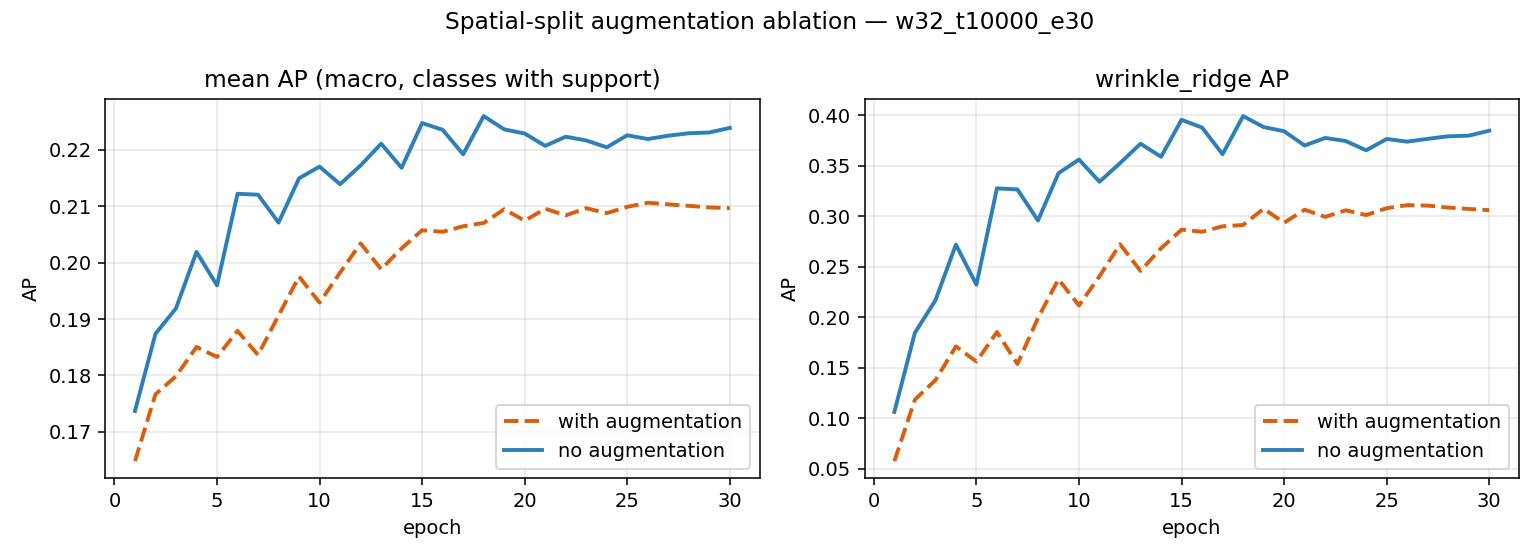
\includegraphics[width=0.85\columnwidth,keepaspectratio]{figures/MR/spatial_w32_t10000_e30_val_ap.png}
\caption{Validation AP across training epochs under the leakage-free spatial split (macro mean over classes with support, left; \texttt{wrinkle\_ridge}, right). The no-augmentation arm dominates at every epoch on both metrics.}
\label{fig:spatial_rerun}
\end{figure}

\paragraph{Definitive model.}
The definitive model is SmallUNet with $w=32$, FocalDice, residual shortcuts, bottleneck dropout ($p=0.3$), trained \emph{without} augmentation for 30 epochs on the full dataset. One caveat applies to this synthesis across studies: Studies 1--2 were run with augmentation enabled, before Study 3 established it is harmful; their selected components are architectural choices not expected to interact strongly with augmentation, but re-confirming those rankings in the no-augmentation regime remains the natural next experiment.

\subsection{Qualitative evaluation}
\label{sec:mr_qualitative}

Metrics alone do not reveal \emph{how} a model fails, so the ablations are complemented by a visual comparison on identical validation tiles for the BCEDice baseline and the definitive model. The ridge comparison (Fig.~\ref{fig:qualitative_ridge}) shows that the metric gains of the definitive model correspond to a real, visible improvement in the completeness of the recovered ridge network, with errors concentrated on thin, low-contrast segments. The crater comparison (Fig.~\ref{fig:qualitative_crater}), conversely, makes the saturation argument of Sect.~\ref{sec:mr_dataset} concrete: the ground truth fills entire tiles, so predicting ``everywhere'' is trivially correct.

\begin{figure}[htbp!]
\centering
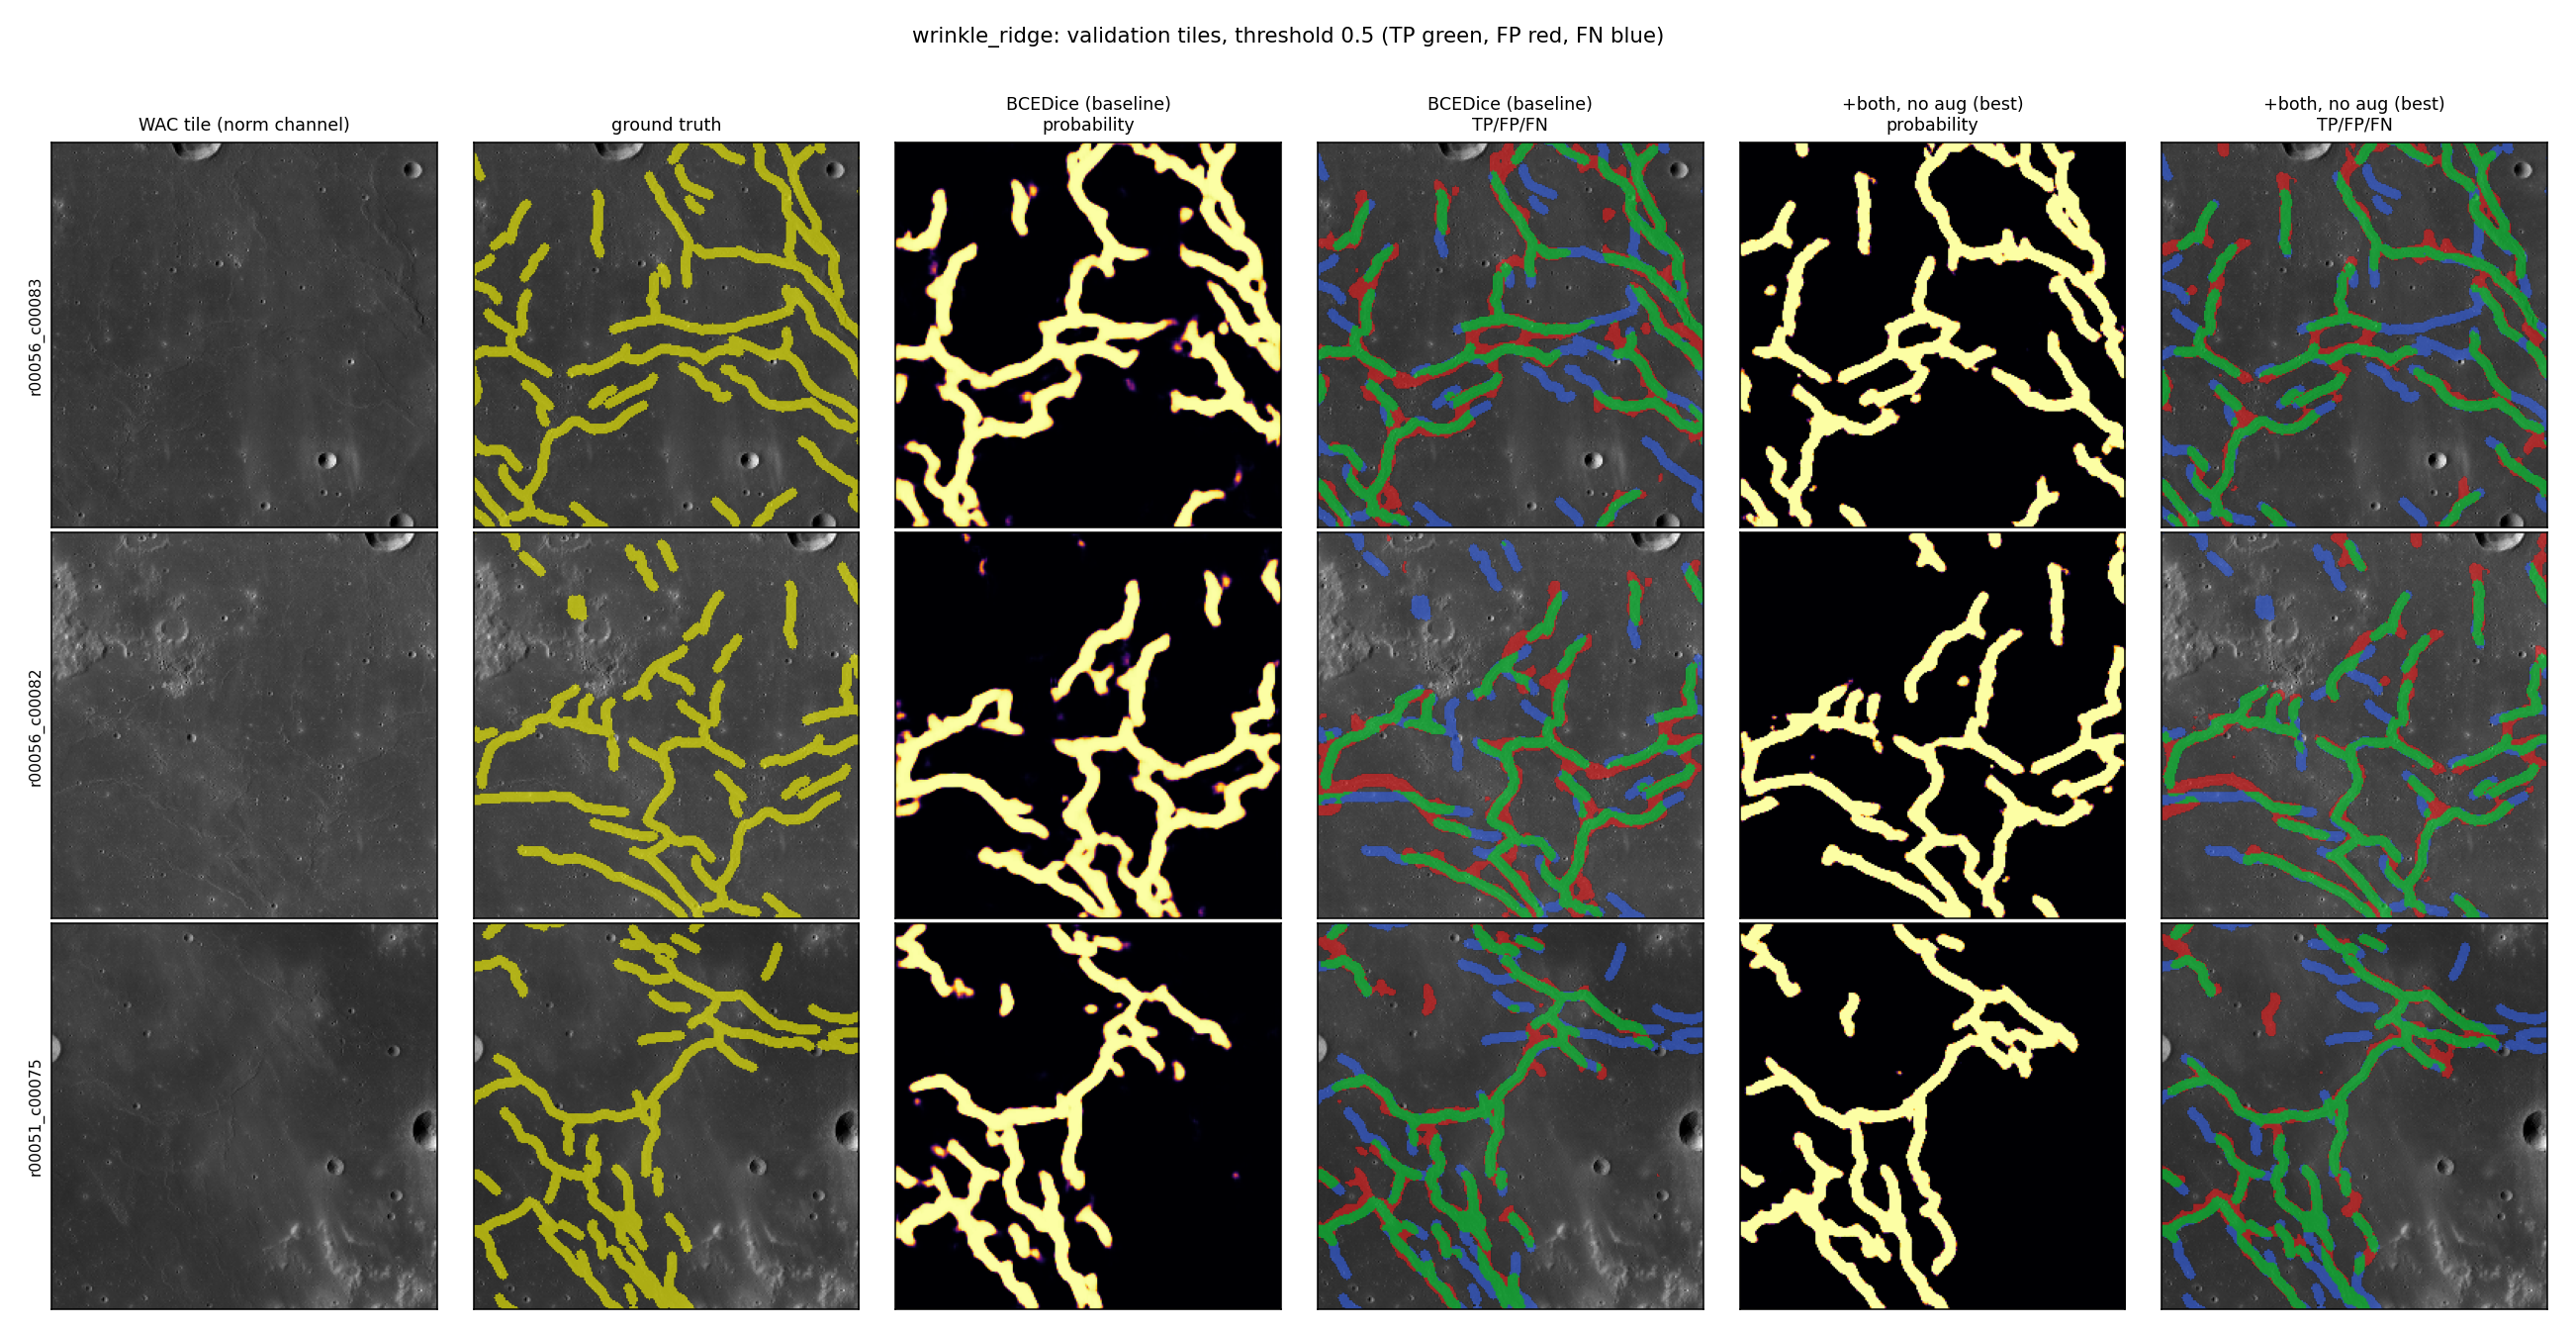
\includegraphics[width=0.85\columnwidth,keepaspectratio]{figures/MR/qualitative_wrinkle_ridge.png}
\caption{Wrinkle-ridge qualitative comparison on three validation tiles (TP green, FP red, FN blue). Both models recover the topology of the ridge network; the definitive model (+both, no augmentation) produces visibly more complete coverage and fewer false positives than the BCEDice baseline.}
\label{fig:qualitative_ridge}
\end{figure}

\begin{figure}[htbp!]
\centering
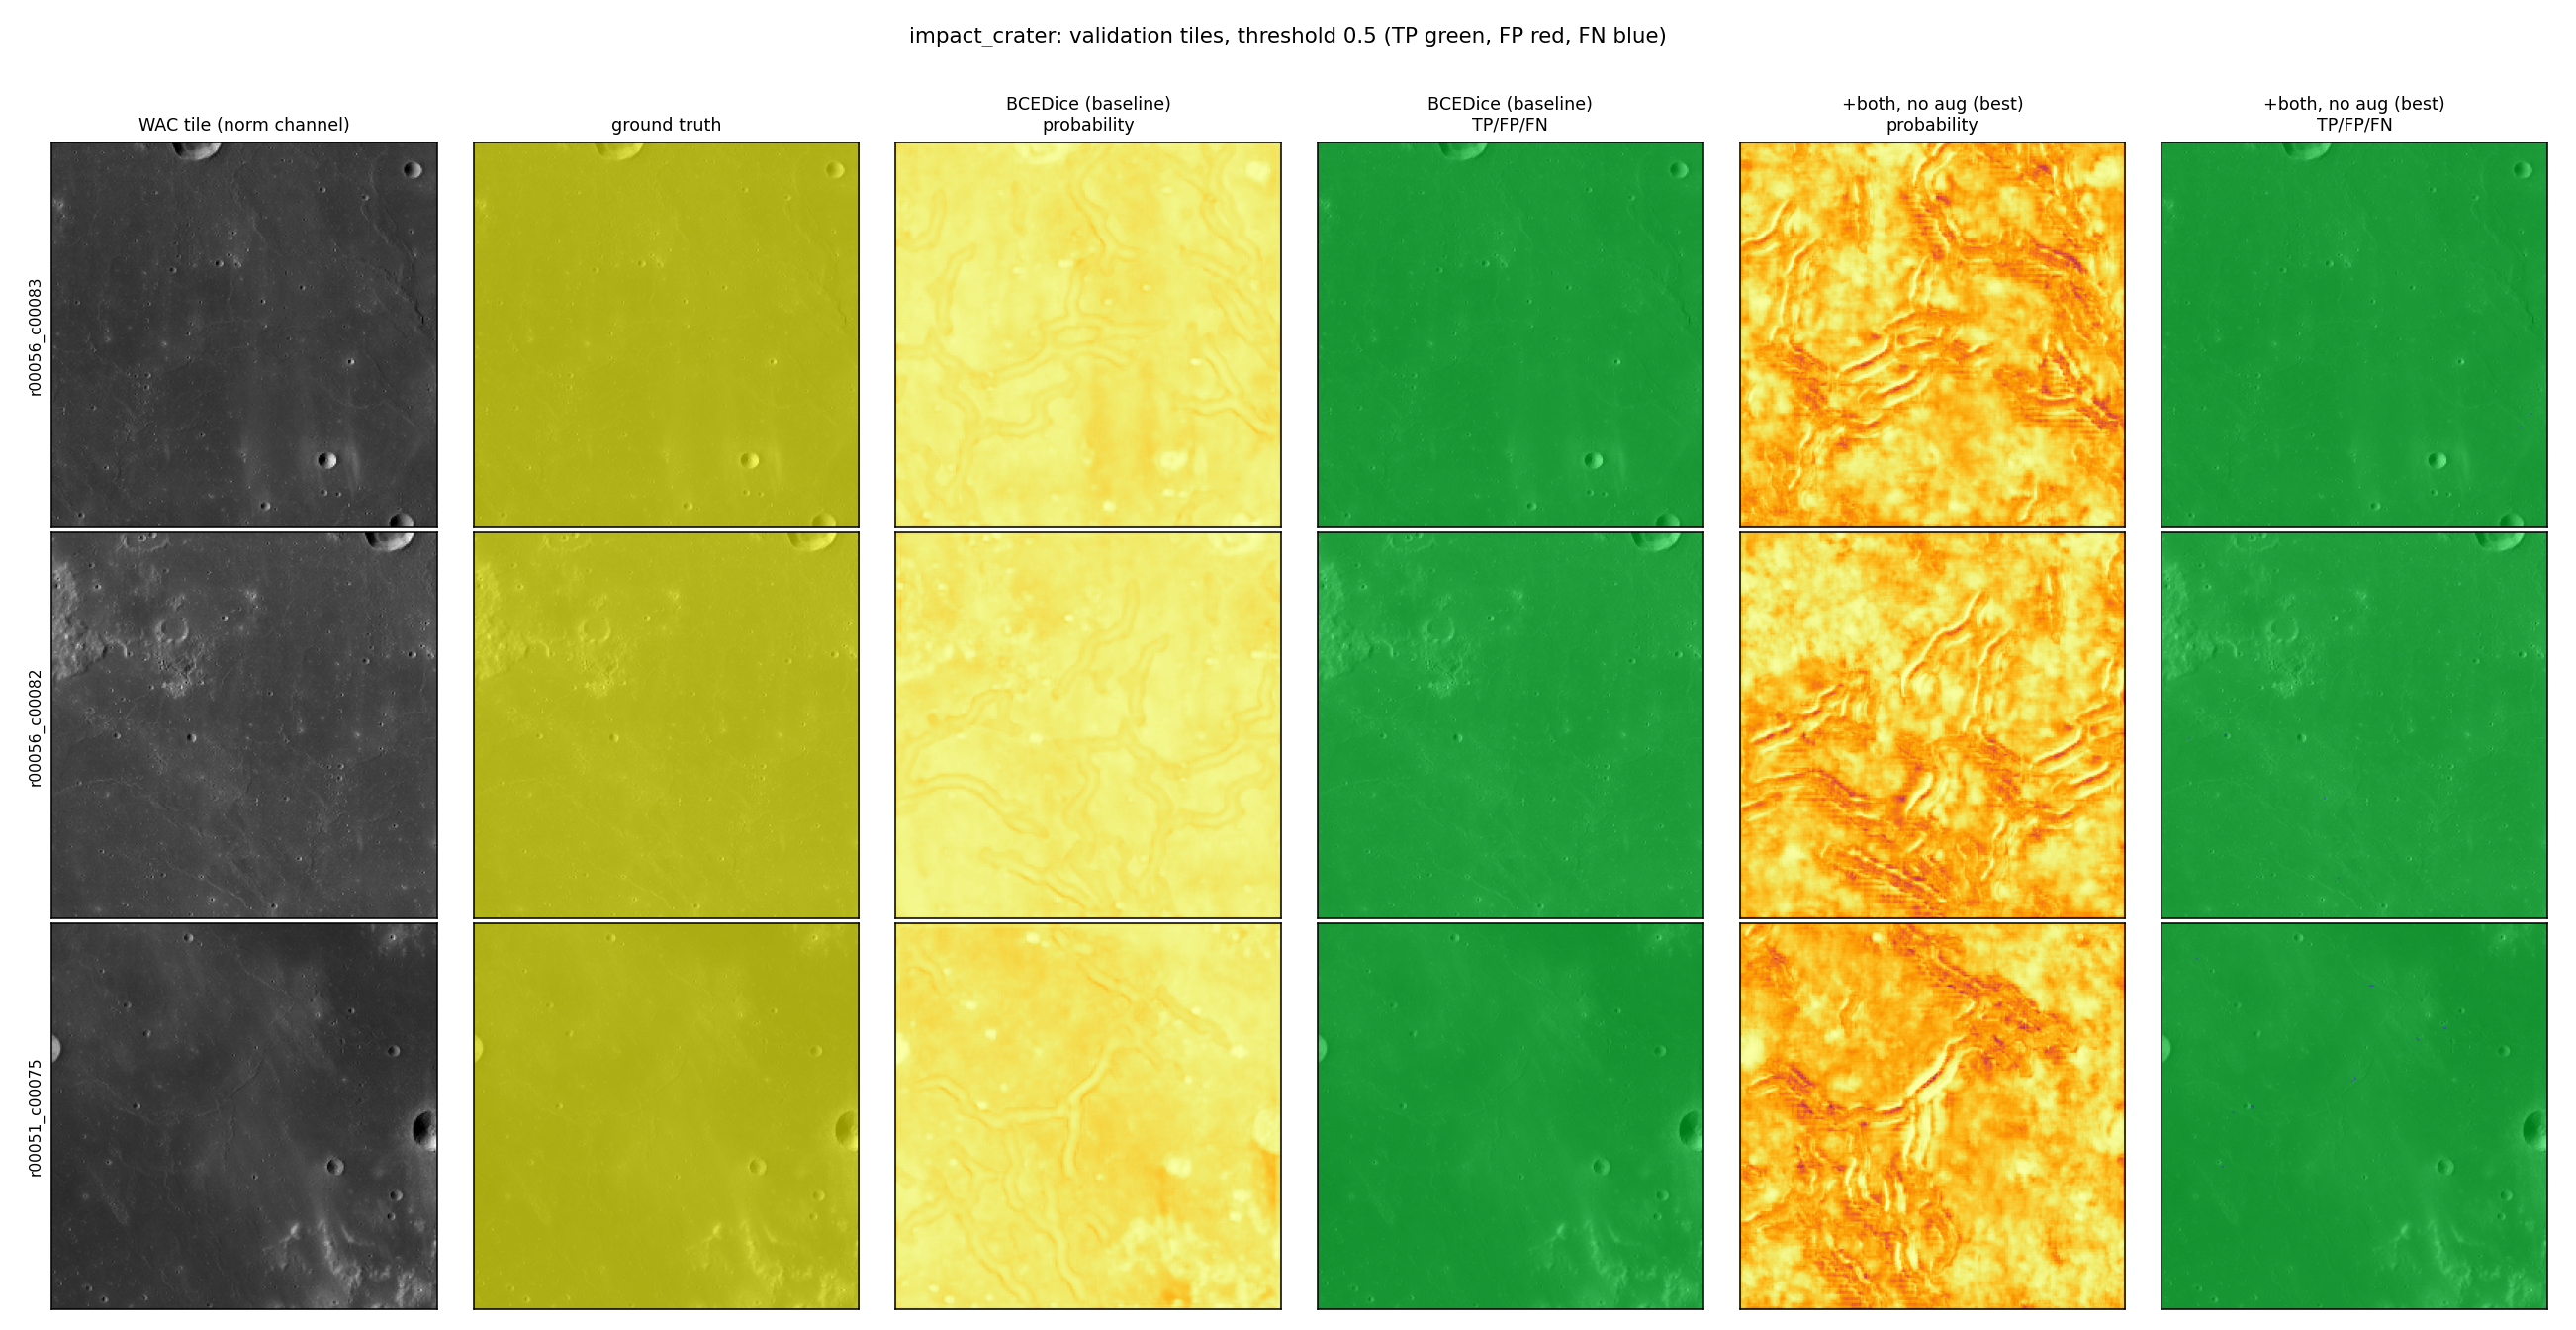
\includegraphics[width=0.85\columnwidth,keepaspectratio]{figures/MR/qualitative_impact_crater.png}
\caption{Impact-crater qualitative comparison on the same tiles. The ground truth covers the \emph{entire} tile (cf.\ the 82.1\% pixel prevalence and 50.7\% fully-covered tiles of Table~\ref{tab:prevalence}), so a prediction of ``everywhere'' is trivially correct: direct visual evidence that the crater channel behaves as a near-coverage layer and that crater AP must be read against its 0.821 chance baseline.}
\label{fig:qualitative_crater}
\end{figure}


\section{Object detection with YOLOv8}
\label{sec:yolo}

The third learned formulation treats lunar features as objects to be localised with bounding boxes. YOLO \citep{redmon2016yolo} frames detection as a single regression pass --- box coordinates and class probabilities are predicted simultaneously in one forward pass, avoiding the region-proposal stage of two-stage detectors and making the method orders of magnitude faster. We use YOLOv8n \citep{jocher2023yolov8} (3.0M parameters, anchor-free decoupled head), COCO-pretrained and fine-tuned on the lunar tiles. Box targets are generated from the semantic mask channels by connected-component labelling, with per-class size gates discarding degenerate components (minimum side 5\,px; maximum side 100\,px for craters, 300\,px otherwise).

\paragraph{Experiment 1: all seven classes.}
The box-level class distribution is even more skewed than the pixel-level one: impact craters contribute 382{,}122 of 399{,}691 instances (95.5\%), wrinkle ridges 16{,}133 (4.0\%), and the remaining five classes below 0.2\% each, with all boxes small relative to the image (most spanning ${\sim}5\%$ of its side). Trained for 100 epochs on this dataset, the model converges stably (a transient loss spike near epoch 90 is the cosine-annealing restart) but fails to generalise beyond the dominant class: recall grows only to ${\sim}0.05$, concentrated on craters. Full label statistics and training diagnostics for both experiments are collected in Appendix~\ref{app:yolo}.

\paragraph{Experiment 2: craters removed.}
Excluding the impact-crater class leaves 17{,}486 instances dominated by wrinkle ridges (92.6\%). Training on this reduced six-class dataset is markedly more stable --- all losses decrease smoothly, training and validation remain closely aligned, and recall (${\sim}0.043$) is now spread across the six rare classes rather than concentrated on craters. Class imbalance, not model capacity, was the primary limiting factor of the first experiment; even a simple class-removal curation significantly improves convergence.

\subsection{A decoupled per-group ensemble}
\label{sec:yolo_ensemble}

The natural next step is to decouple the problem entirely: instead of one seven-class model, a small ensemble of specialised detectors, each trained only on morphologically similar classes so that high-frequency features cannot overwhelm the gradient signal of rare ones. Classes are grouped by geometry --- a two-dimensional (areal) group $f_1$ (craters, pits, mare patches, Apollo sites) and a one-dimensional (curvilinear) group $f_2$ (ridges, scarps, rilles) --- and within each group the dominant class receives a dedicated single-class detector while the rest share a second one, yielding four YOLOv8n models. Figure~\ref{fig:yolo_ensemble_cm} shows the validation confusion matrices of the two multi-class members: within a morphological group the rare classes are separable once the dominant class is removed, with confusion against background as the main residual error mode.

\begin{figure}[htbp!]
\centering
\begin{subfigure}[b]{0.48\columnwidth}
    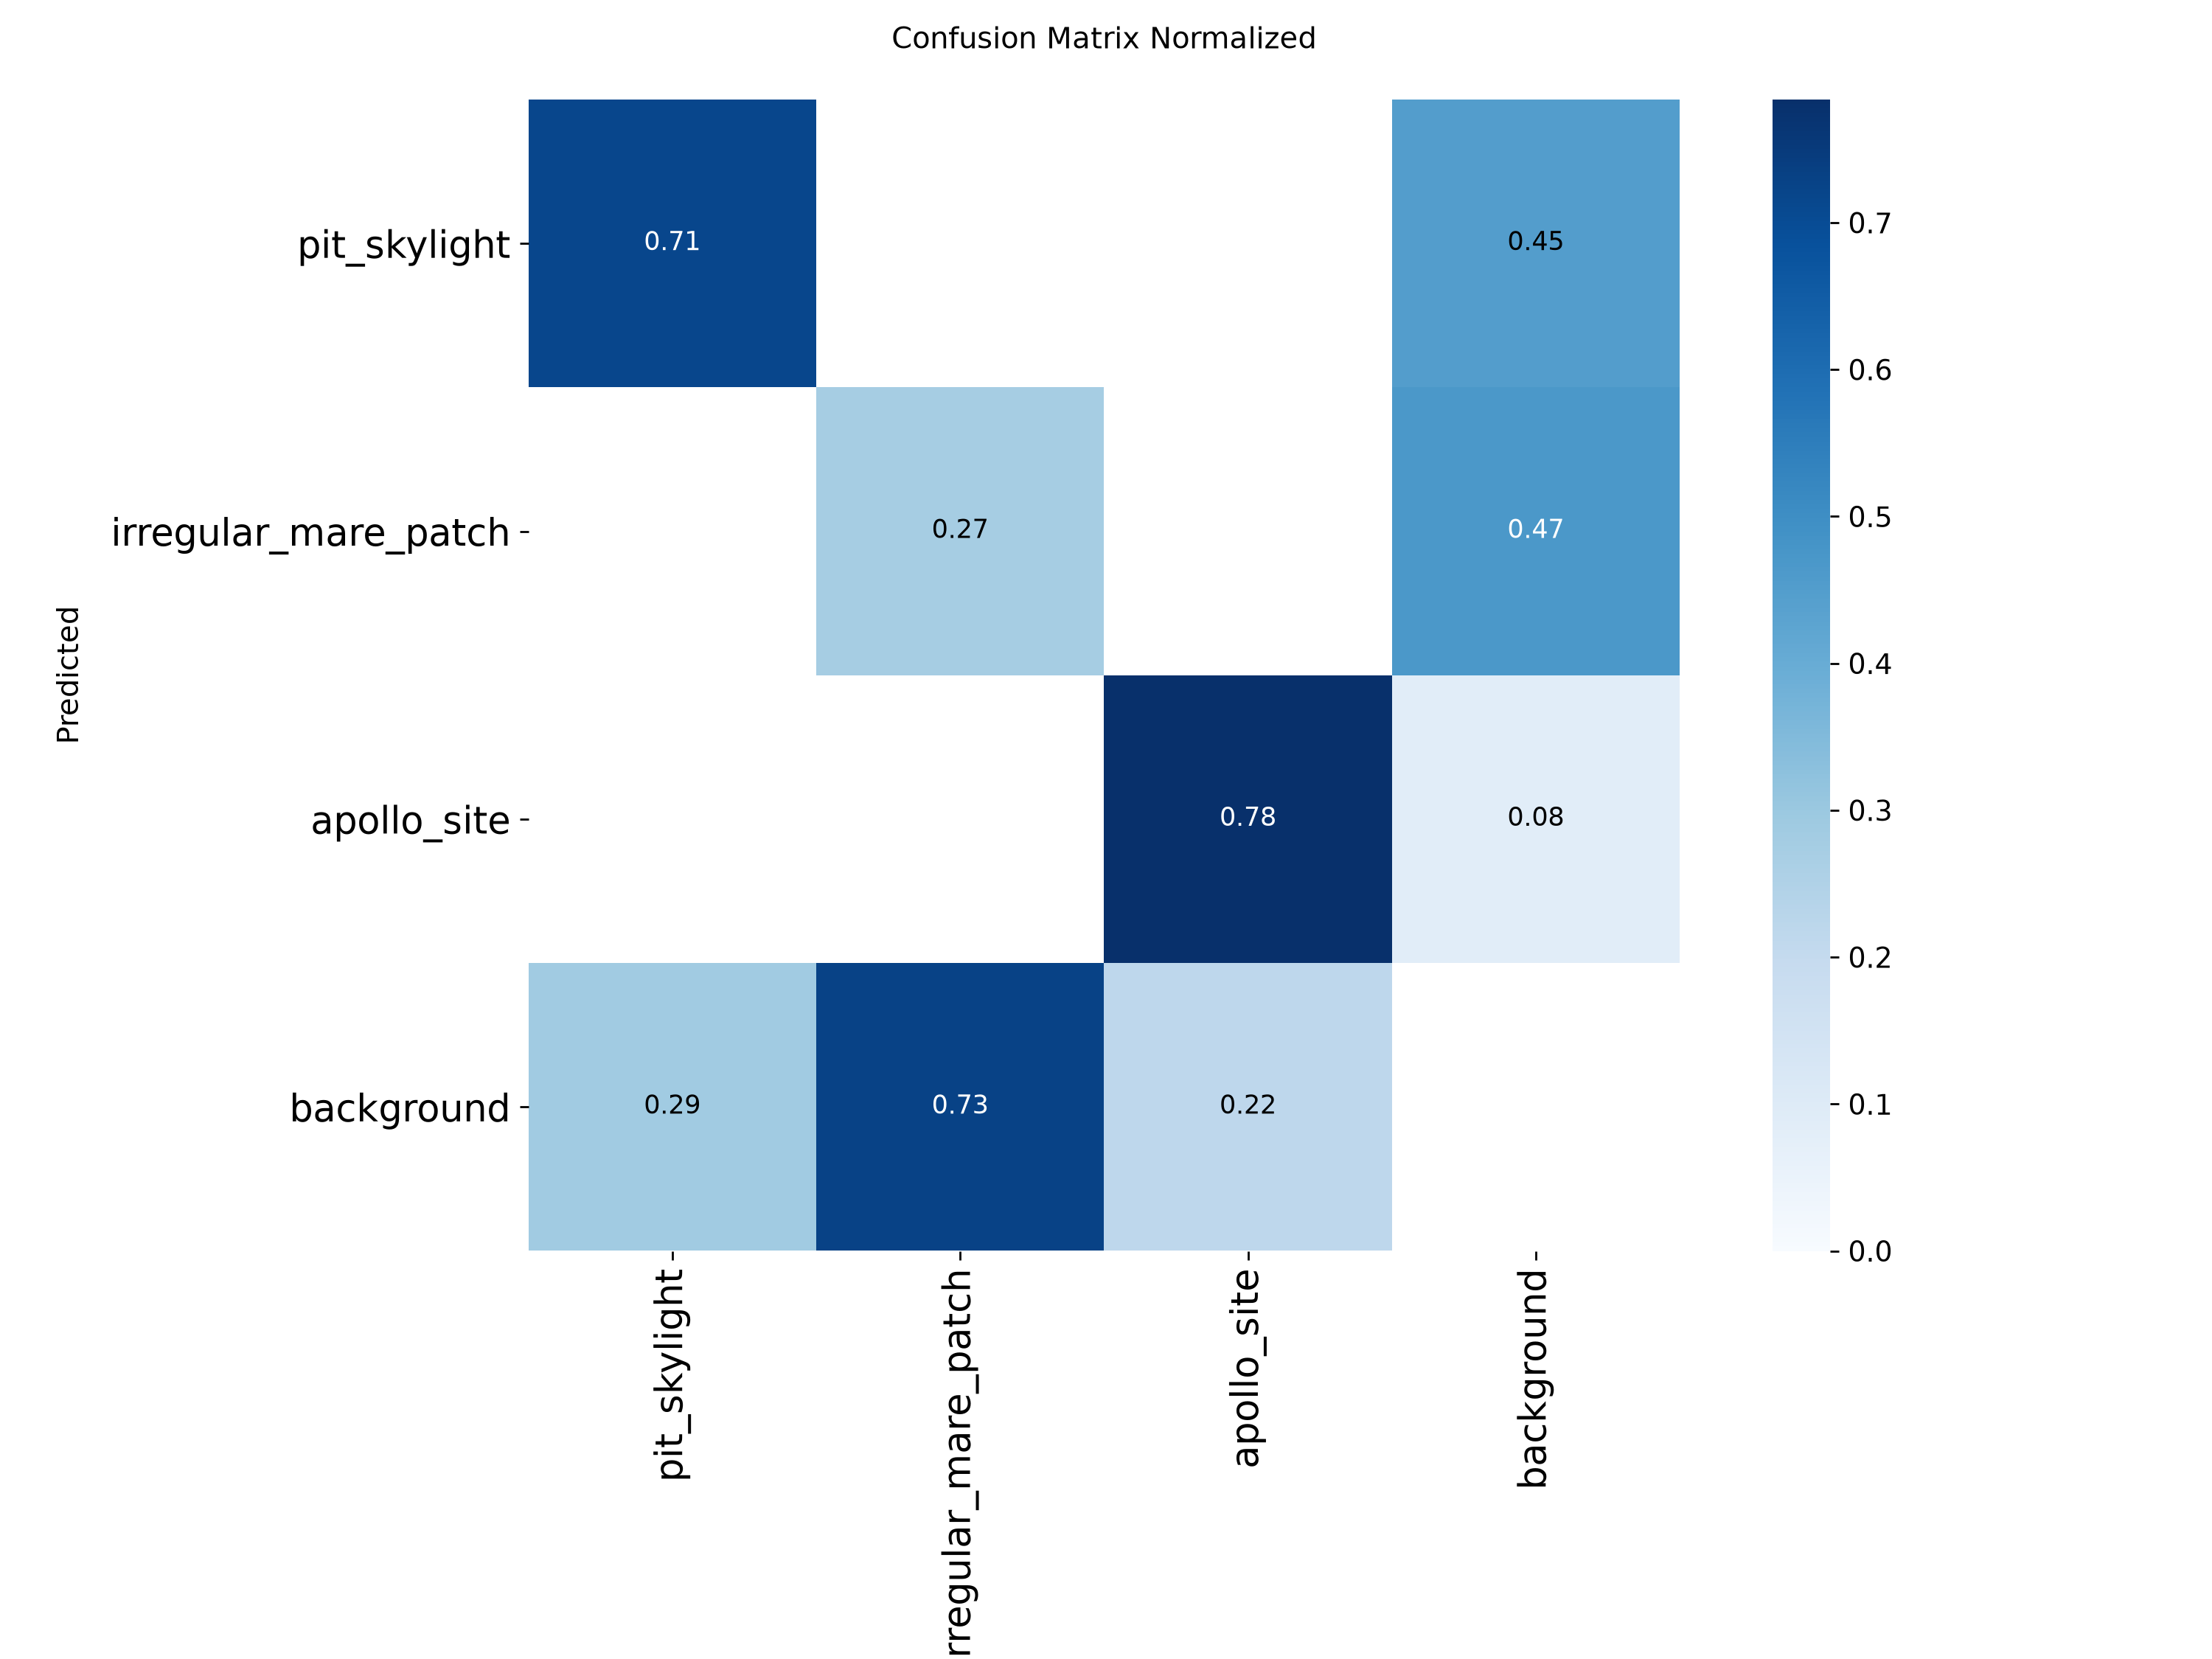
\includegraphics[width=\textwidth]{figures/YOLO/YOLO_f1.2_matrix.png}
    \caption{$f_1$ group model.}
\end{subfigure}
\hfill
\begin{subfigure}[b]{0.48\columnwidth}
    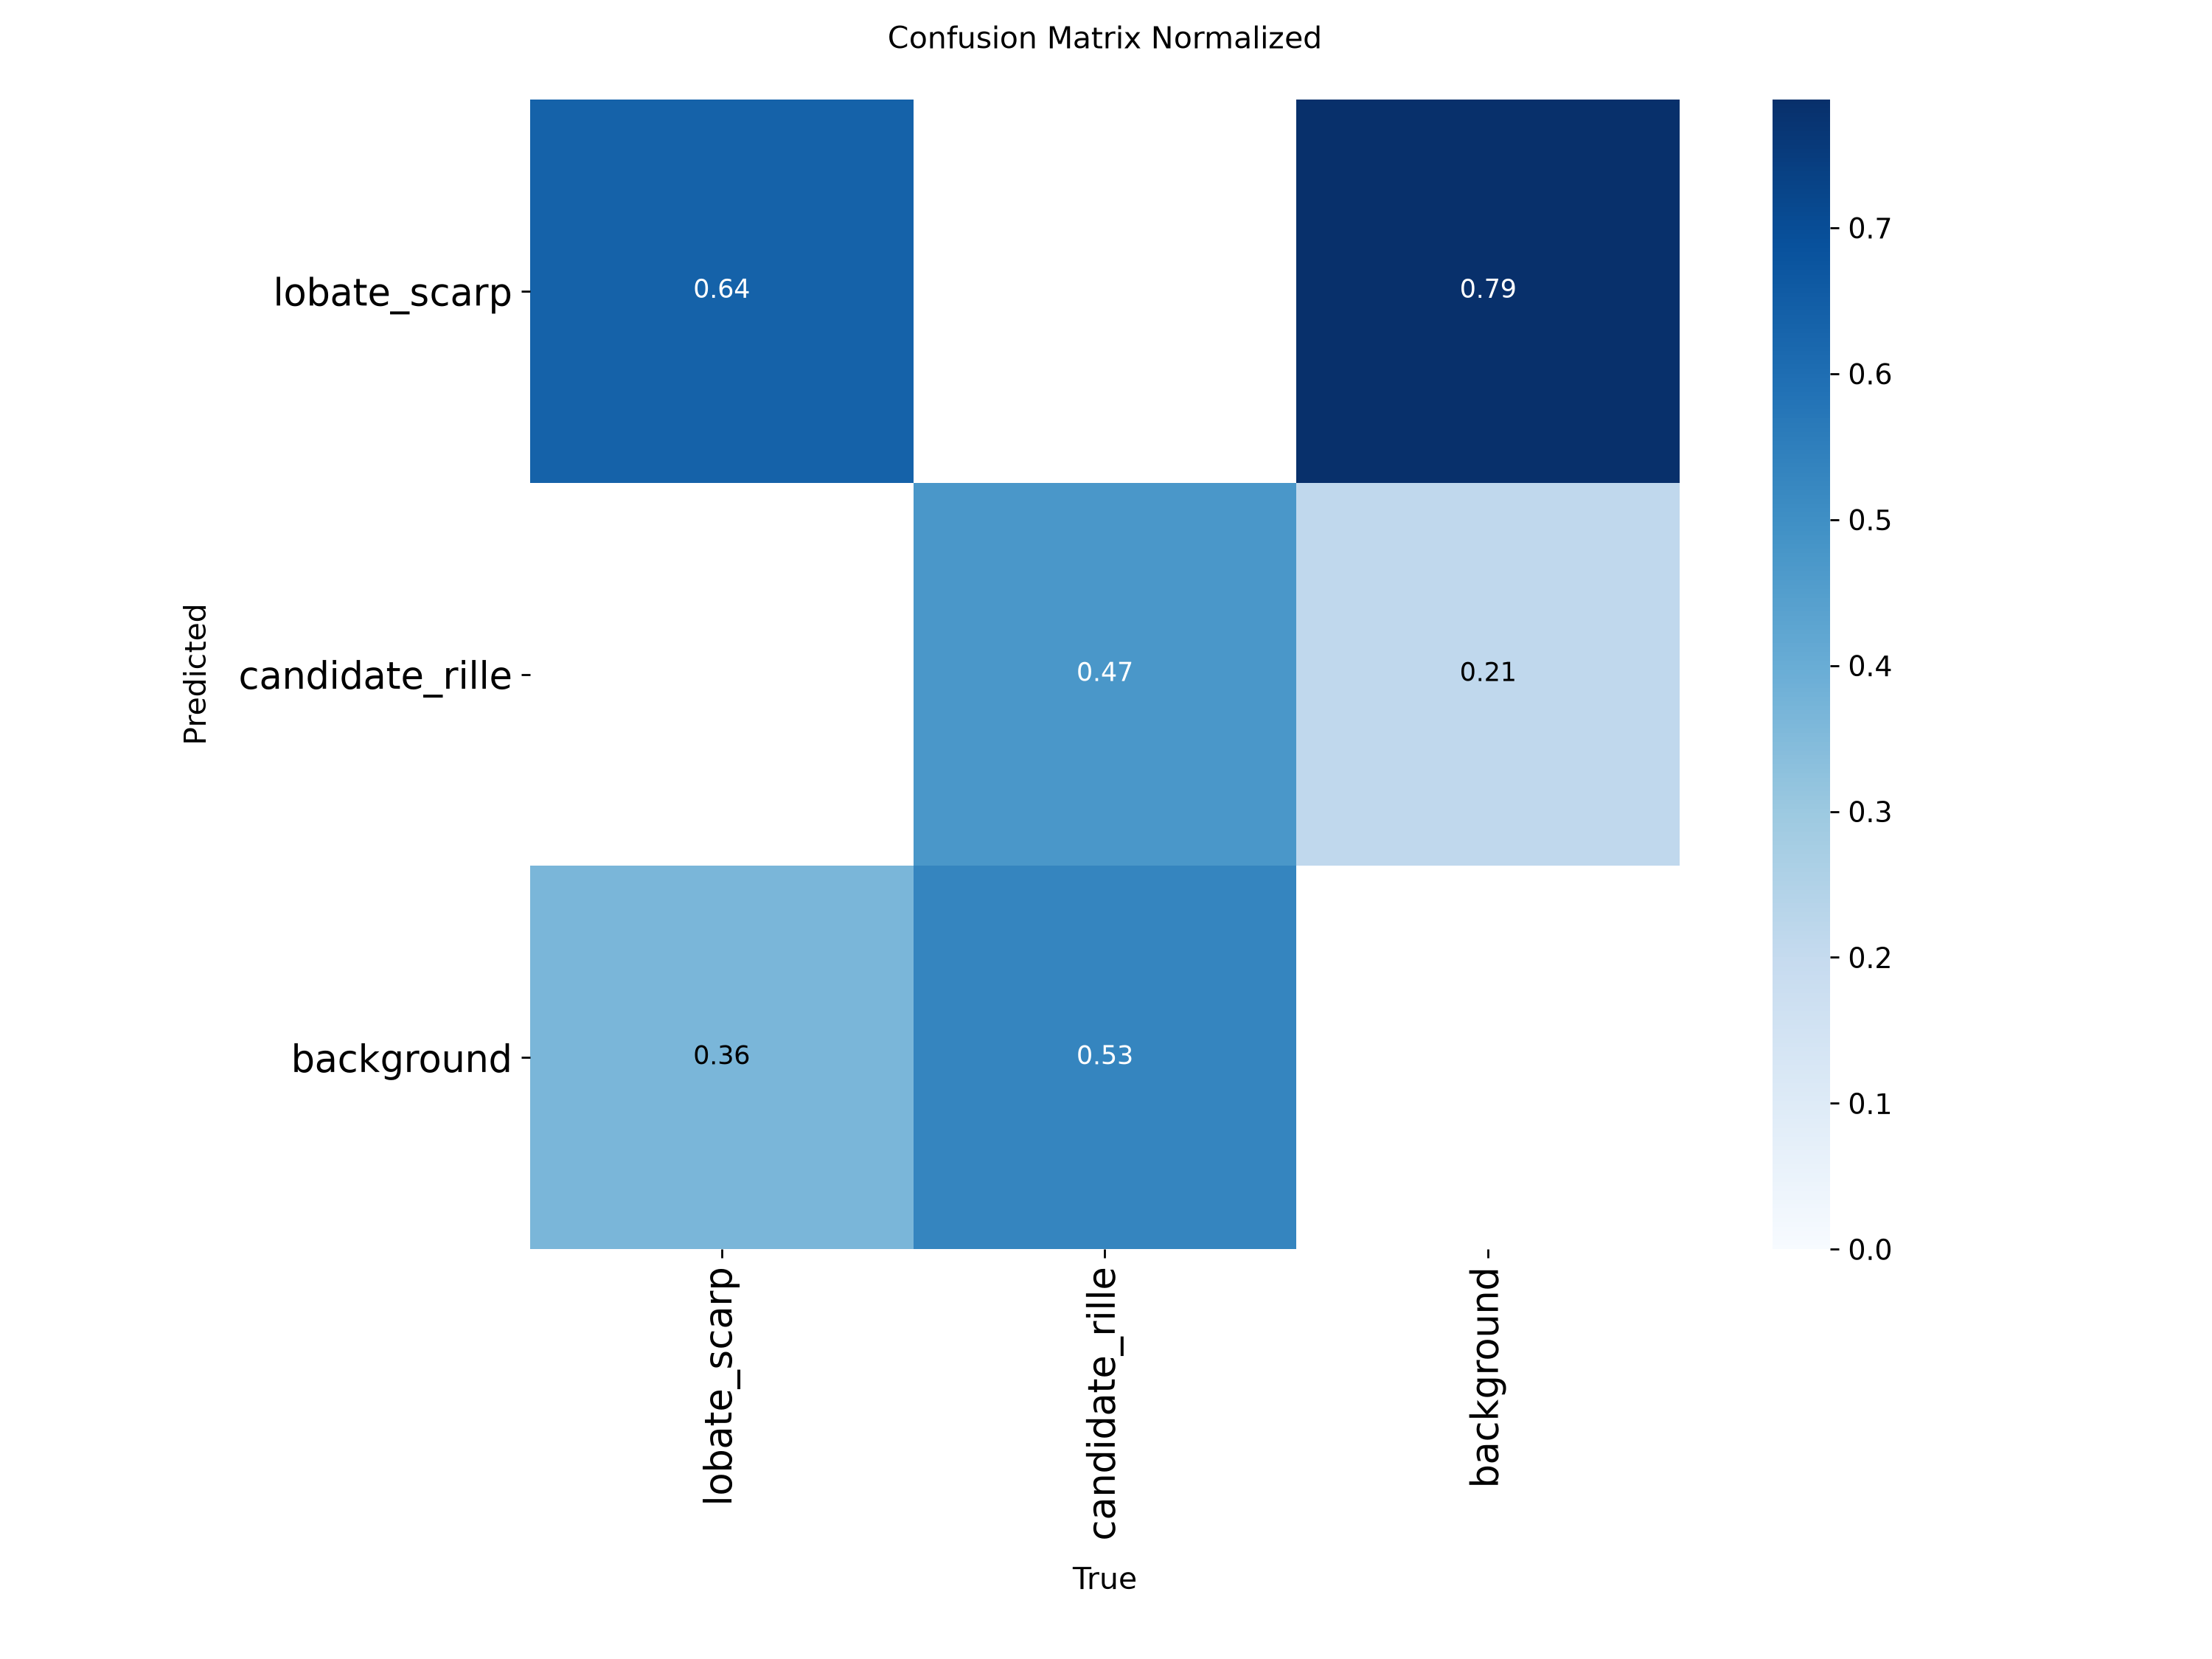
\includegraphics[width=\textwidth]{figures/YOLO/YOLO_f2.2_matrix.png}
    \caption{$f_2$ group model.}
\end{subfigure}
\caption{Normalised validation confusion matrices of the two multi-class ensemble members (random-split protocol).}
\label{fig:yolo_ensemble_cm}
\end{figure}

On the random-split protocol used during development, the training-run validation scores of the two single-class members reached mAP50 $\approx0.9$, while the multi-class members remained much lower (${\approx}0.50$ for $f_1$, ${\approx}0.25$ for $f_2$). These development scores are not comparable to the numbers of Sect.~\ref{sec:comparison}: they are measured on a random split over 50\%-overlapping tiles, on datasets restricted to feature-bearing tiles, and at a different training budget. Sect.~\ref{sec:split_study} disentangles exactly this, by retraining the ensemble's two single-class detectors under both split protocols at matched budget.


\FloatBarrier

\section{Head-to-head comparison under the shared protocol}
\label{sec:comparison}

This section contains the central results of the paper: all four methods, reduced to per-class binary masks, scored with identical metrics on the identical spatially disjoint validation tiles (Sect.~\ref{sec:metrics_protocol}). The comparison is organised per class, because the two classes with usable supervision pose opposite problems: \texttt{impact\_crater} is nearly saturated (prevalence 0.82) while \texttt{wrinkle\_ridge} is sparse (prevalence 0.0064) but genuinely learnable.

\subsection{Impact crater: the base-rate regime}
\label{sec:comp_crater}

On the full spatial validation set the crater channel covers 82\% of pixels, and a \emph{predict-everything} baseline attains F1 $=0.90$ and IoU $=0.82$ with MCC $=0$. Table~\ref{tab:crater_allval} shows that the SmallUNet essentially reproduces this baseline (F1 $=0.90$, MCC $=0.01$): its high F1 is not evidence of skill --- the network has learned to output the base rate, which on a channel where 50.7\% of tiles contain no negative pixels at all (Table~\ref{tab:prevalence}) is very hard to beat. Any comparison ranking methods by F1 or IoU here would be ranking base-rate reproduction; this is why MCC is the protocol's primary metric.

\begin{table}[htbp]
\centering
\caption{Impact crater, full spatial validation set (per-method calibrated threshold $\tau$). The predict-all row labels every pixel crater. MCC is the primary ranking metric; F1/IoU are dominated by the 0.82 base rate.}
\label{tab:crater_allval}
\resizebox{\columnwidth}{!}{%
\begin{tabular}{lrrrrrr}
\toprule
Method & $\tau$ & Precision & Recall & F1 & IoU & MCC \\
\midrule
YOLOv8 (detection)     & 0.2  & 0.893 & 0.940 & 0.916 & 0.846 & \textbf{0.470} \\
Classical (thr+morph)  & 0.5  & 0.878 & 0.238 & 0.374 & 0.230 & 0.078 \\
SmallUNet (semantic)   & 0.3  & 0.823 & 1.000 & 0.903 & 0.823 & 0.013 \\
Mask R-CNN (instance)  & 0.05 & 0.616 & 0.064 & 0.116 & 0.061 & $-0.166$ \\
\midrule
Predict-all (baseline) & ---  & 0.823 & 1.000 & 0.903 & 0.823 & 0.000 \\
\bottomrule
\end{tabular}
}
\end{table}

Partitioning the validation tiles by crater coverage (Table~\ref{tab:crater_regime}, Fig.~\ref{fig:regime}) shows that the best method \emph{flips} with the regime. On crater-sparse tiles (1--20\% coverage), where craters are countable objects, the instance and detection formulations lead: Mask R-CNN (MCC 0.19) ahead of YOLOv8 (0.16), with the classical baseline modest (0.07) and the SmallUNet at chance. On crater-dense tiles ($\geq$20\%), where the channel is a coverage layer, YOLOv8 keeps a positive signal (0.24) while Mask R-CNN collapses ($-0.11$; such tiles are out of distribution for its instance-target preparation, which skips channels above 20\% coverage, Sect.~\ref{sec:maskrcnn}), and the SmallUNet remains at chance in \emph{both} regimes. One caveat: MCC and F1 at a fixed operating point are sensitive to the calibrated threshold, so absolute values shift with $\tau$; the rankings and the regime flip are stable across the calibration range we scanned.

\begin{table}[htbp]
\centering
\caption{Impact crater by coverage regime (spatial validation split; per-method, per-regime calibrated $\tau$). The preferable formulation flips between regimes.}
\label{tab:crater_regime}
\resizebox{\columnwidth}{!}{%
\begin{tabular}{llrrrr}
\toprule
Regime & Method & $\tau$ & F1 & MCC & Count MAE \\
\midrule
sparse (1--20\%, $n=94$)  & Mask R-CNN & 0.2  & 0.279 & \textbf{0.187} & 82.8 \\
                          & YOLOv8     & 0.05 & 0.253 & 0.159 & 105.5 \\
                          & Classical  & 0.5  & 0.142 & 0.069 & 15.6 \\
                          & SmallUNet  & 0.3  & 0.176 & $-0.000$ & 24.0 \\
\midrule
dense ($\geq$20\%, $n=192$) & YOLOv8     & 0.1  & 0.947 & \textbf{0.240} & 12.6 \\
                          & Classical  & 0.5  & 0.387 & 0.031 & 49.3 \\
                          & SmallUNet  & 0.3  & 0.945 & $-0.001$ & 4.9 \\
                          & Mask R-CNN & 0.05 & 0.132 & $-0.111$ & 41.3 \\
\bottomrule
\end{tabular}
}
\end{table}

\begin{figure}[htbp!]
\centering
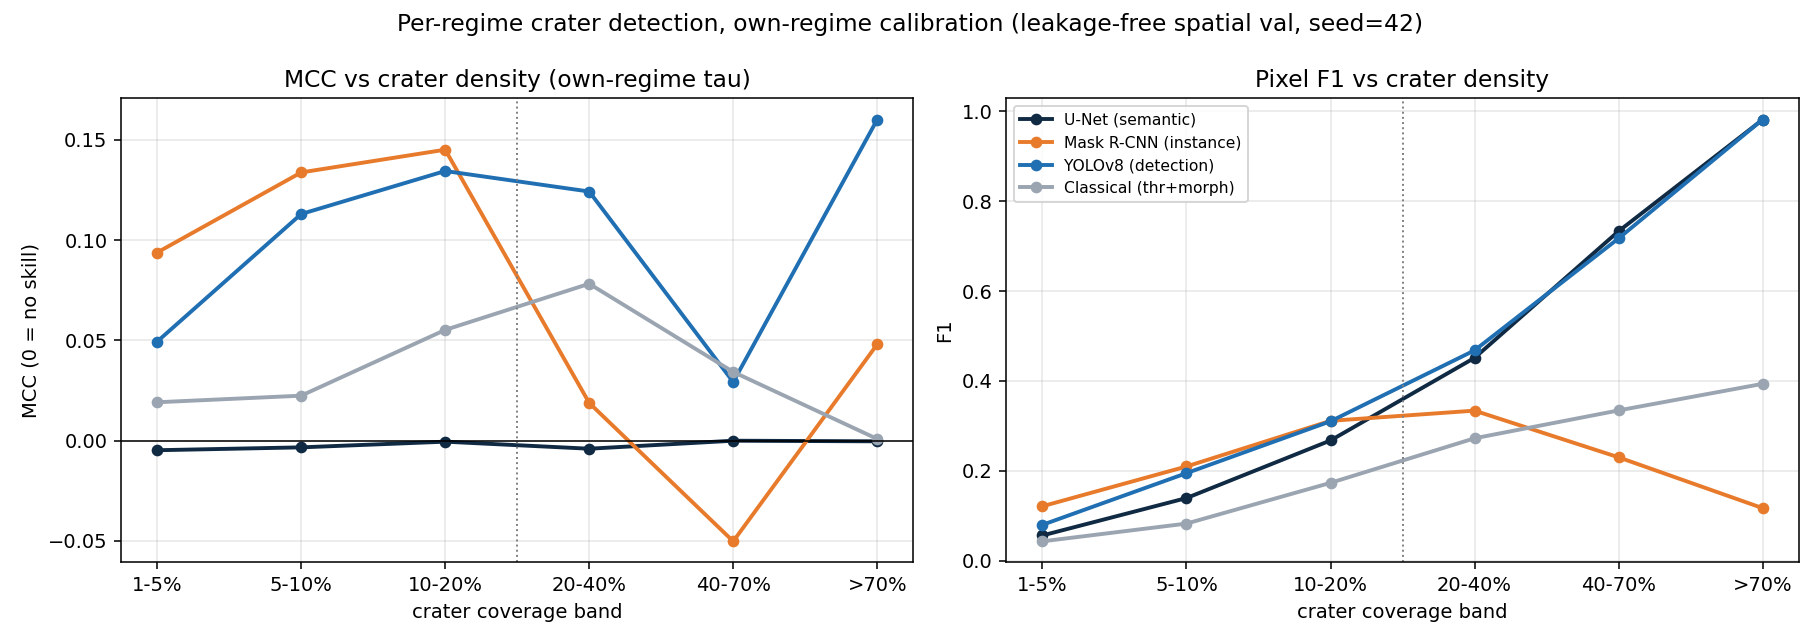
\includegraphics[width=\columnwidth,keepaspectratio]{figures/comparison/fig_regime.png}
\caption{Impact-crater comparison by coverage regime on the spatial validation split. Left: MCC (skill over base rate); right: F1 for reference. The ranking flips between regimes, and the SmallUNet sits at MCC $\approx0$ in both --- its high F1 on dense tiles is base-rate reproduction, not detection skill.}
\label{fig:regime}
\end{figure}

\subsection{Wrinkle ridge: the class with genuine signal}
\label{sec:comp_ridge}

Wrinkle ridges are the mirror image of craters: prevalence 0.0064, so chance-level performance is near zero and any positive score reflects learned structure. The comparison runs on the 524 ridge-bearing tiles of the spatial validation split (210 calibration / 314 test); the SmallUNet entry is the definitive no-augmentation spatial checkpoint of Sect.~\ref{sec:mr_augmentation}, the YOLOv8 entry the committed ridge-focused six-class model, and the classical entry the Sato filter of Sect.~\ref{sec:classical}.

\begin{table}[htbp]
\centering
\caption{Wrinkle ridge, spatial validation split (314 test tiles, per-method calibrated $\tau$). Prevalence 0.0064: chance-level MCC is 0, and the predict-all baseline collapses.}
\label{tab:ridge}
\resizebox{\columnwidth}{!}{%
\begin{tabular}{lrrrrrr}
\toprule
Method & $\tau$ & Precision & Recall & F1 & MCC & ms/tile \\
\midrule
SmallUNet (semantic)   & 0.25 & 0.527 & 0.409 & \textbf{0.460} & \textbf{0.452} & 20 \\
Mask R-CNN (instance)  & 0.5  & 0.414 & 0.352 & 0.380 & 0.366 & 1130 \\
YOLOv8 (detection)     & 0.01 & 0.063 & 0.228 & 0.099 & 0.076 & 10 \\
Classical (Sato)       & 0.05 & 0.021 & 0.392 & 0.040 & $-0.028$ & 29 \\
\midrule
Predict-all (baseline) & ---  & 0.026 & 1.000 & 0.050 & 0.000 & --- \\
\bottomrule
\end{tabular}
}
\end{table}

\begin{figure}[htbp!]
\centering
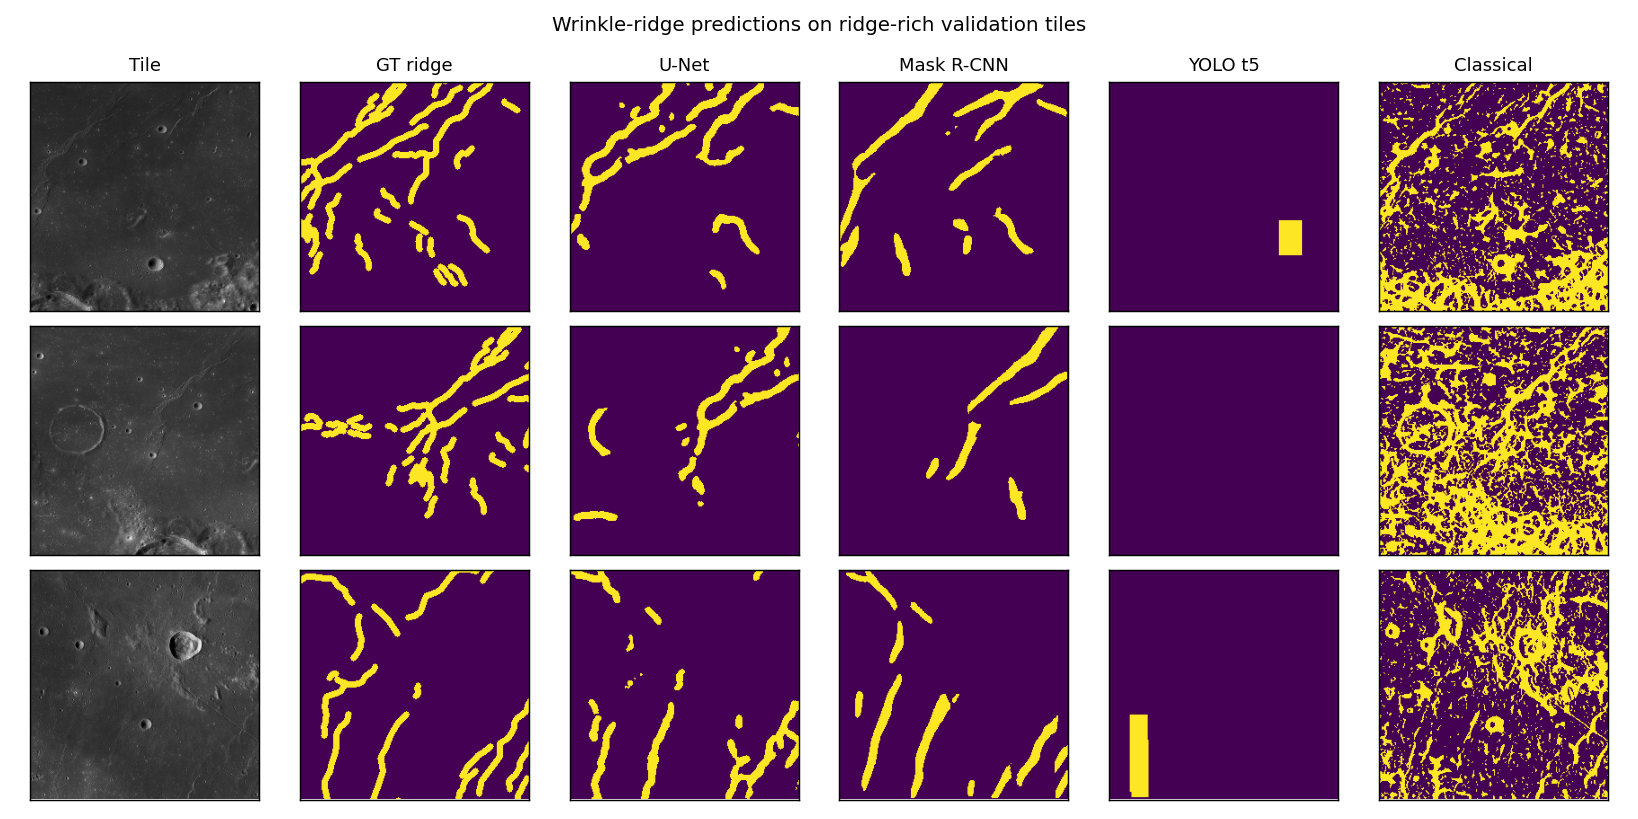
\includegraphics[width=\columnwidth,keepaspectratio]{figures/comparison/fig_ridge_qualitative.png}
\caption{Qualitative ridge predictions on common validation tiles (columns: image, ground truth, then one column per method). The SmallUNet recovers the connected ridge network; Mask R-CNN recovers the strongest segments; YOLOv8 boxes are coarse; the Sato filter responds to every elongated bright structure, ridge or not.}
\label{fig:ridge_qual}
\end{figure}

The ranking reverses relative to the sparse-crater regime: \textbf{SmallUNet (MCC 0.452) $>$ Mask R-CNN (0.366) $\gg$ YOLOv8 (0.076) $>$ Sato ($\approx$ chance)} (Table~\ref{tab:ridge}, Fig.~\ref{fig:ridge_qual}). The two pixel-supervised models are far ahead, consistent with the nature of the class: ridges are thin, extended, and connected --- pixel supervision describes them well, whereas a diagonal ridge fills a small fraction of its own bounding box. The SmallUNet additionally beats Mask R-CNN at ${\sim}1/60$th of the inference cost, and the context-free classical filter stays at chance. Together with Sect.~\ref{sec:comp_crater} this yields the central per-class conclusion: \emph{semantic segmentation wins where dense pixel supervision exists; instance detection wins for sparse countable objects; nothing wins on a saturated channel.}

\subsection{Effect of the split protocol: a controlled study}
\label{sec:split_study}

To quantify what the split choice does to a reported number, we retrained \emph{identical} single-class YOLOv8n detectors (image size 256, batch 16, 40 epochs, identical seeds and hyperparameters) on datasets built by the same box-extraction code, changing \emph{only} the split: random 80/20 tile split versus spatial block split, with comparable training volumes in both arms (crater: 5\,659 vs.\ 5\,077 tiles; ridge: 2\,339 vs.\ 2\,202). We report each model on its own validation set, plus a decomposition row --- the random-split model evaluated on the \emph{spatial} validation tiles --- which separates the training-side from the evaluation-side component of the leakage.

\begin{table}[htbp]
\centering
\caption{Split-protocol study: identical YOLOv8n detectors, identical budget (40 epochs), different train/validation split. ``Random $\to$ spatial'' evaluates the random-split model on the spatial validation tiles.}
\label{tab:split_study}
\resizebox{\columnwidth}{!}{%
\begin{tabular}{llrrr}
\toprule
Class & Protocol & mAP50 & Precision & Recall \\
\midrule
impact crater & random tile split (own val) & 0.122 & 0.217 & 0.222 \\
              & spatial split (own val)     & 0.106 & 0.206 & 0.201 \\
              & random $\to$ spatial val    & 0.129 & 0.228 & 0.219 \\
\midrule
wrinkle ridge & random tile split (own val) & 0.146 & 0.297 & 0.191 \\
              & spatial split (own val)     & 0.077 & 0.203 & 0.130 \\
              & random $\to$ spatial val    & 0.117 & 0.278 & 0.162 \\
\bottomrule
\end{tabular}
}
\end{table}

Both classes replicate the effect, with strongly class-dependent size (Table~\ref{tab:split_study}). For wrinkle ridges the protocol choice alone nearly doubles the reported score: mAP50 0.146 (random) against 0.077 (spatial) for an identical model, budget, and pipeline. The decomposition row separates the contributions: on \emph{identical} validation tiles the random-trained model outscores the spatial-trained one (0.117 vs.\ 0.077) --- a training-side contamination benefit of $+0.040$, since its training set contains tiles overlapping the validation blocks --- while the remaining $+0.029$ (0.146 vs.\ 0.117) is the evaluation-side component, the random protocol's own validation tiles sharing half their pixels with training tiles. For craters the total effect is much smaller (0.122 vs.\ 0.106): the near-saturated channel offers little memorisable detail that is not already ubiquitous.

Extending the ridge pair to 150 epochs (Fig.~\ref{fig:split_divergence}) confirms the budget dependence: the random-split curve climbs monotonically (0.146 at epoch 40, 0.217 at 150, still rising) while the spatial-split curve saturates before epoch 40 in the 0.06--0.08 band, so the gap \emph{grows} with training --- from $\times1.9$ to $\times2.6$ --- as additional epochs memorise near-duplicate content while genuine generalisation stopped improving long before. Two consequences follow. First, random-split scores on this dataset are not comparable to spatial ones, and the discrepancy is largest exactly where detection genuinely works; development-time scores quoted at large budgets under random splits (Sect.~\ref{sec:yolo_ensemble}) therefore overstate generalisation increasingly with budget. Second, the honest absolute level matters for Sect.~\ref{sec:comp_ridge}: the dedicated single-class ridge detector under the spatial protocol (mAP50 0.077) is fully consistent with the six-class model's shared-protocol showing (MCC 0.076) --- YOLO's weakness on ridges is a property of the box representation on curvilinear features, not an artefact of one training run.

\begin{figure}[htbp!]
\centering
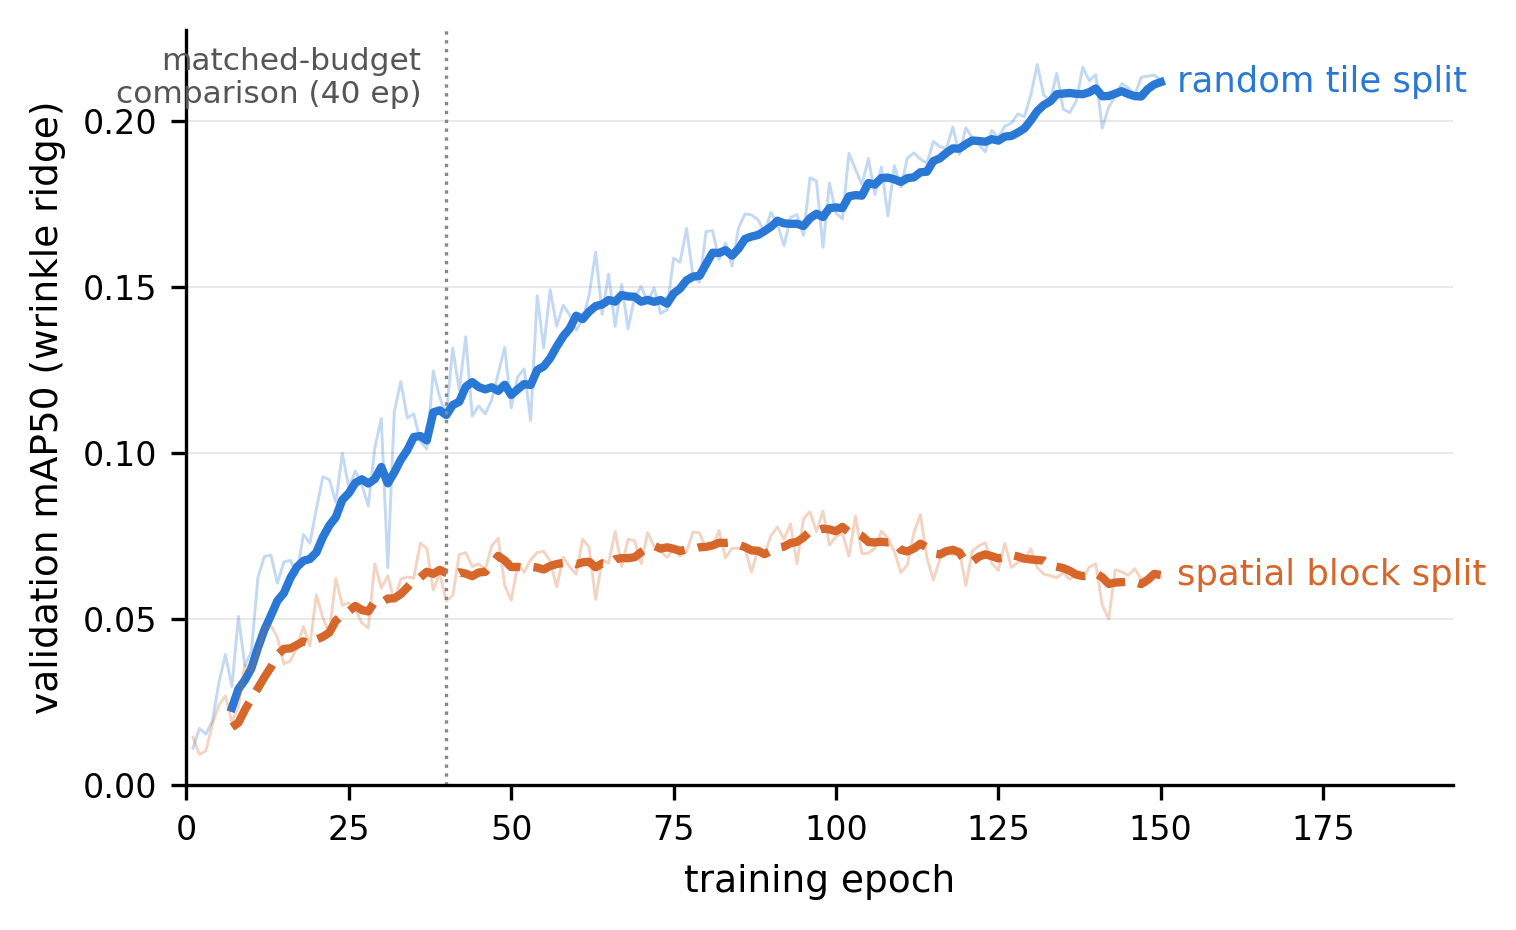
\includegraphics[width=\columnwidth,keepaspectratio]{figures/comparison/fig_split_divergence.png}
\caption{Validation mAP50 of the single-class wrinkle-ridge detector over 150 epochs under the two split protocols (thin: per-epoch; thick: 7-epoch rolling mean; dotted: the matched-budget comparison of Table~\ref{tab:split_study}). The random-split curve keeps climbing as training memorises near-duplicate tiles; the spatial-split curve --- true generalisation --- plateaus before epoch 40. A leaky protocol plus a long training run can report an arbitrarily inflated score.}
\label{fig:split_divergence}
\end{figure}

\subsection{Trade-offs beyond accuracy}
\label{sec:tradeoffs}

Accuracy is one axis; Table~\ref{tab:ridge} also reports cost. Mask R-CNN pays ${\sim}1.1$\,s per tile on CPU --- a full south-pole pass takes over an hour, versus about a minute for the SmallUNet and YOLOv8 and seconds for the classical baseline. Data-preparation effort differs as sharply: the segmentation networks consume the semantic masks directly, while both detection methods depend on a semantic-to-instance conversion whose noise propagates into training targets (Sect.~\ref{sec:maskrcnn}). Interpretability runs in the opposite direction: every classical parameter has physical meaning, detector boxes are auditable object by object, and dense probability maps require post-hoc threshold calibration. None of these axes changes the per-class accuracy ranking, but they decide deployability: for survey-scale mapping of ridge-like features the SmallUNet offers the best accuracy-per-cost, while for counting sparse objects Mask R-CNN's lead costs two orders of magnitude more compute.


\section{Application: mapping the lunar south pole}
\label{sec:southpole}

As a transfer test, the trained pipelines are deployed on the lunar south pole --- a region of high scientific and operational interest that is geologically distinct from the volcanic Marius Hills training domain. South-pole imagery from the same LRO WAC source is tiled identically, producing 3\,639 tiles. No feature catalogue exists for this region, so everything in this section is a transfer \emph{diagnostic}, not an accuracy measurement (Sect.~\ref{sec:metrics_protocol}).

\paragraph{Semantic segmentation transfer.}
Each tile is preprocessed with the training-time CLAHE + Sobel pipeline and passed through the definitive SmallUNet checkpoint; Table~\ref{tab:south_pole_stats} reports the aggregated confidence statistics, Fig.~\ref{fig:south_pole_best} the most confident tile per class, and Appendix~\ref{app:southpole} the underlying per-class distribution diagnostics. The model assigns high crater probability across the entire region (average per-tile maximum 0.863) --- expected behaviour given the near-saturated crater layer learned in training, and not to be over-interpreted as precise crater delineation (Sect.~\ref{sec:comp_crater}). Two classes, \texttt{wrinkle\_ridge} and \texttt{candidate\_rille}, show very low average probabilities but anomalously high global maxima (1.000 and 0.480): rare but confident predictions on a few tiles rather than diffuse activation. The weak performance on rare classes reflects the combination of domain shift and the near-absence of supervision for those classes even in the training region.

\begin{table}[htbp]
\centering
\caption{SmallUNet south-pole inference (3\,639 tiles). Avg.\ Max.\ Prob.\ is the mean, over tiles, of the per-tile maximum predicted probability; Global Max the highest probability in any tile.}
\label{tab:south_pole_stats}
\resizebox{\columnwidth}{!}{%
\begin{tabular}{lrrr}
\toprule
Class & Avg.\ Max.\ Prob. & Global Max & Status \\
\midrule
\texttt{impact\_crater}       & 0.863 & 1.000 & $\checkmark$ detected \\
\texttt{lobate\_scarp}        & 0.060 & 0.303 & weak \\
\texttt{pit\_skylight}        & 0.051 & 0.202 & weak \\
\texttt{irregular\_mare\_patch} & 0.040 & 0.215 & weak \\
\texttt{apollo\_site}         & 0.040 & 0.183 & weak \\
\texttt{candidate\_rille}     & 0.006 & 0.480 & sparse \\
\texttt{wrinkle\_ridge}       & 0.001 & 1.000 & sparse \\
\bottomrule
\end{tabular}
}
\end{table}

\begin{figure}[htbp!]
\centering
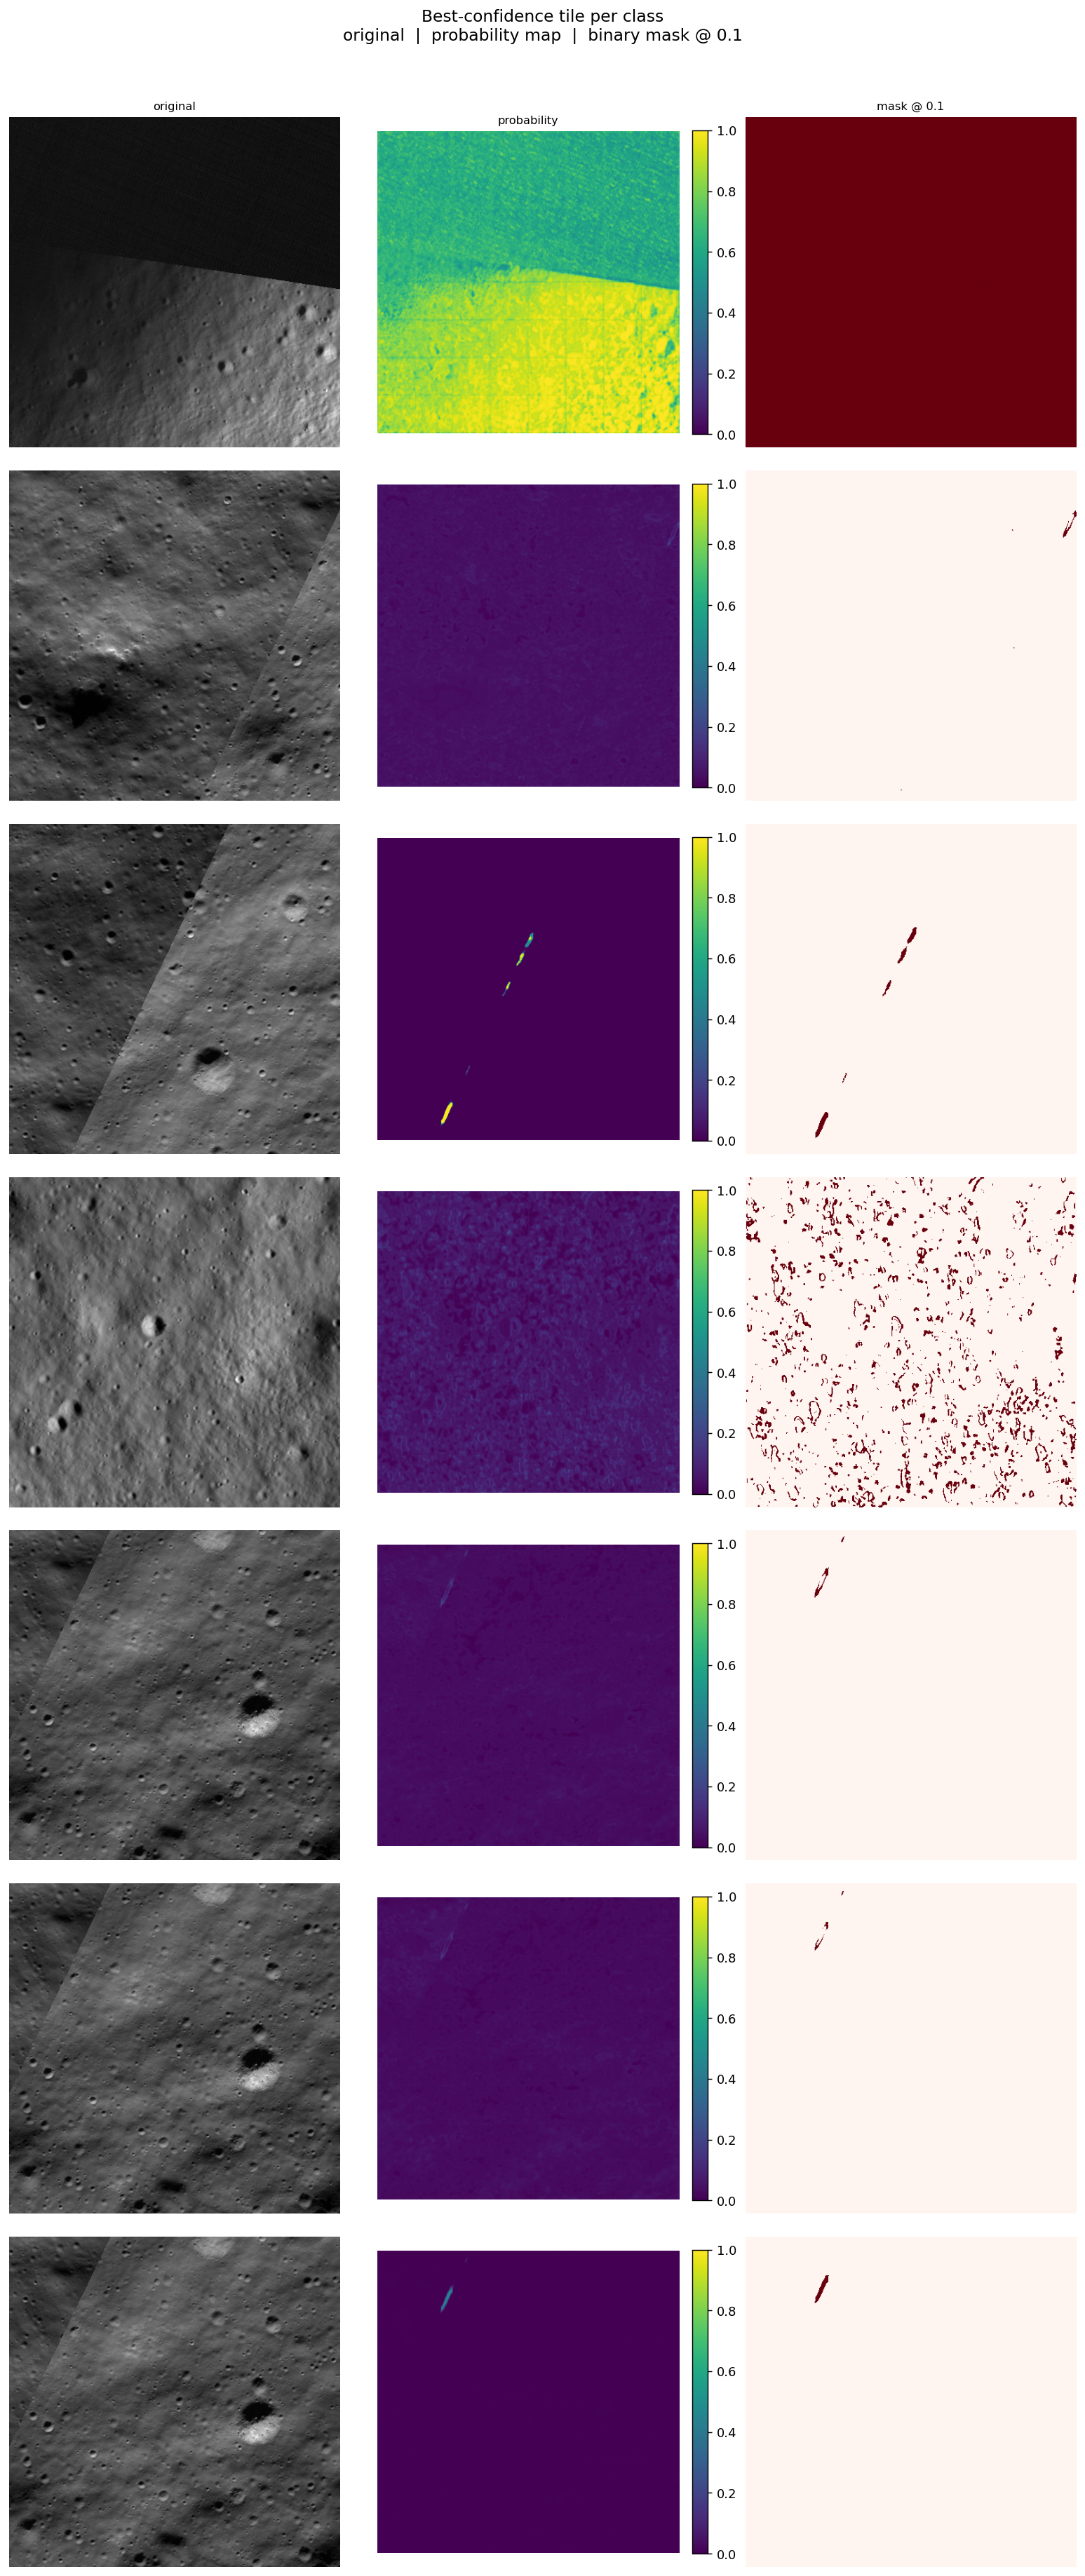
\includegraphics[width=0.85\columnwidth,keepaspectratio]{figures/MR/diagnostics_best_tiles.png}
\caption{Best-detected tile per class on the south pole imagery. Each panel shows the LRO WAC tile overlaid with the predicted probability map for the class with the highest maximum confidence in that tile. Overlays use a \emph{relative} threshold (top fraction of each tile's probabilities), so coloured regions for the weak classes are candidate locations, not confident detections.}
\label{fig:south_pole_best}
\end{figure}

At survey scale the inference runs through a decoupled pipeline: tiles are streamed through the network, each probability cube is serialised immediately to compressed \texttt{.npz} storage, and statistics are aggregated in a second pass over the stored arrays.

\paragraph{Detection-level transfer.}
The two detection formulations were deployed on the same tiles, and their disagreement is as instructive as their agreement. The YOLOv8 ensemble (Sect.~\ref{sec:yolo_ensemble}), at confidence $\geq0.5$, predicts a population that is overwhelmingly craters (98.0\% of detections), then wrinkle ridges (1.4\%) and lobate scarps (0.6\%) --- a plausible composition for heavily cratered highland terrain, consistent with the segmentation diagnostics. Mask R-CNN at its nominal threshold (0.5) instead returns only 52 instances in the entire region, \emph{all} ridges and \emph{zero} craters; craters emerge only as the threshold drops (188 detections at $\tau=0.2$, 8\,176 at 0.1, 104\,871 at 0.05). This is the domain-shift signature of a detector whose crater recall was already weak in-distribution (Sect.~\ref{sec:maskrcnn}): its crater confidence collapses below the nominal operating point on unfamiliar terrain. With no ground truth, no single composition can be validated --- but read together, the three formulations triangulate what a single pipeline cannot: segmentation and YOLOv8 agree on a crater-dominated region with rare linear tectonic features, while Mask R-CNN's threshold sweep shows which conclusions are hostage to confidence calibration under domain shift. In an unlabelled region, cross-method agreement is the only available currency of trust.


\section{Discussion and conclusions}
\label{sec:conclusions_global}

Four formulations of lunar feature recognition --- classical image processing, semantic segmentation, instance segmentation, and single-stage detection --- were compared on the same data, the same spatially disjoint split, and the same metrics. The principal conclusions:

\begin{enumerate}
    \item \textbf{There is no single best architecture; the class regime decides.} On the sparse, genuinely supervised wrinkle-ridge class the pixel-supervised models dominate (SmallUNet MCC 0.452 $>$ Mask R-CNN 0.366 $\gg$ YOLOv8 0.076 $>$ classical $\approx$ chance): thin connected structures fit pixel supervision and fit bounding boxes poorly. On crater-sparse tiles the ranking flips and the detection formulations lead (Mask R-CNN 0.19, YOLOv8 0.16, SmallUNet $\approx0$). Matching the output representation to the geometry of the class matters more than architectural sophistication within a family.

    \item \textbf{A saturated label channel cannot be won, only diagnosed.} The crater channel covers 82\% of pixels; a predict-everything baseline attains F1 $=0.90$, and the SmallUNet's seemingly excellent crater F1 reproduces exactly that baseline (MCC $\approx0$ in every regime). Prevalence-robust metrics are not a refinement here but a necessity.

    \item \textbf{The evaluation protocol moves numbers more than the architecture does.} Retraining identical detectors under a random versus a spatial split (Sect.~\ref{sec:split_study}) quantifies the leakage induced by 50\%-overlapping tiles, and the augmentation study reached its conclusion only after being re-run leakage-free. Split geometry, metric choice, and threshold calibration must be fixed \emph{before} architectures are compared; several apparent contradictions between the single-method experiments of this project dissolved once their numbers were re-read under a common protocol.

    \item \textbf{Cost and interpretability separate methods that accuracy does not.} Mask R-CNN's sparse-regime lead costs ${\sim}1.1$\,s per tile against 10--20\,ms for YOLOv8 and the SmallUNet and ${\sim}1$\,ms for the classical baseline --- at survey scale, the difference between minutes and hours per region. The classical baseline never wins on accuracy, but it defines the floor a learned method must beat and remains the only fully inspectable pipeline.

    \item \textbf{Method-specific lessons survive the shared protocol.} For Mask R-CNN, mask quality and detection quality decouple (Dice 0.77 on matched objects against mAP@0.5 $\approx1\%$): the bottleneck is proposal recall on noisy instance targets. For the SmallUNet, geometric augmentation is harmful on directionally biased planetary terrain, an effect that persists under the leakage-free split. For YOLOv8, isolating the dominant class (95.5\% of instances) is the single most effective intervention, motivating the decoupled per-group ensemble.

    \item \textbf{Unlabelled deployment needs independent cross-checks.} On the south pole, the segmentation diagnostics and YOLOv8 agree on the composition (craters dominant, linear tectonic features rare), while Mask R-CNN's threshold sweep --- zero craters at its nominal operating point, $10^5$ at $\tau=0.05$ --- shows that any single-pipeline composition is hostage to confidence calibration under domain shift. Agreement between independent pipelines, not single-pipeline confidence, is the currency of trust in unlabelled regions.
\end{enumerate}

Taken together, the study argues that for planetary datasets with extreme prevalence structure, the productive question is not ``which network is best'' but ``which output representation matches each feature class, under an evaluation protocol that cannot be gamed by the base rate'' --- and it provides a reusable such protocol, with all four methods reproducible from the shared repository.

\begin{acknowledgements}
      The Marius Hills and south pole tile datasets were prepared for the Laboratory of Computational Physics (mod.~B) course of the Physics of Data programme, University of Padova. Part of the training runs used GPU resources provided by the CloudVeneto infrastructure.
\end{acknowledgements}


\FloatBarrier

\begin{thebibliography}{}

\bibitem[He et al.(2016)]{he2016resnet} He, K., Zhang, X., Ren, S., \& Sun, J. 2016,
       in Proc.\ IEEE Conf.\ on Computer Vision and Pattern Recognition (CVPR), 770

\bibitem[He et al.(2017)]{he2017maskrcnn} He, K., Gkioxari, G., Doll\'ar, P., \& Girshick, R. 2017,
       in Proc.\ IEEE Int.\ Conf.\ on Computer Vision (ICCV), 2961

\bibitem[Jocher et al.(2023)]{jocher2023yolov8} Jocher, G., Chaurasia, A., \& Qiu, J. 2023,
       Ultralytics YOLOv8, https://github.com/ultralytics/ultralytics

\bibitem[LCP(2026)]{mariusdata} Laboratory of Computational Physics, UniPD 2026,
       Marius Hills lunar feature dataset: pre-processed NPZ tiles

\bibitem[Lin et al.(2017)]{lin2017fpn} Lin, T.-Y., Doll\'ar, P., Girshick, R., He, K., Hariharan, B., \& Belongie, S. 2017,
       in Proc.\ IEEE Conf.\ on Computer Vision and Pattern Recognition (CVPR), 2117

\bibitem[Lin et al.(2017)]{lin2017focal} Lin, T.-Y., Goyal, P., Girshick, R., He, K., \& Doll\'ar, P. 2017,
       in Proc.\ IEEE Int.\ Conf.\ on Computer Vision (ICCV)

\bibitem[Loshchilov \& Hutter(2019)]{loshchilov2019adamw} Loshchilov, I., \& Hutter, F. 2019,
       in Int.\ Conf.\ on Learning Representations (ICLR)

\bibitem[NASA(2023)]{nasa2023southpole} NASA 2023,
       Artemis and the Lunar South Pole: ShadowCam Imaging of Permanently Shadowed Regions

\bibitem[NASA/GSFC(2011)]{pia13523} NASA/GSFC and Arizona State University 2011,
       PIA13523: Lunar South Polar Region, NASA Photojournal

\bibitem[NASA/JPL(2010)]{pia12954} NASA/JPL and University of Arizona 2010,
       PIA12954: A Hole in the Moon (Marius Hills Pit), NASA Photojournal

\bibitem[Redmon et al.(2016)]{redmon2016yolo} Redmon, J., Divvala, S., Girshick, R., \& Farhadi, A. 2016,
       in Proc.\ IEEE Conf.\ on Computer Vision and Pattern Recognition (CVPR), 779

\bibitem[Ronneberger et al.(2015)]{ronneberger2015unet} Ronneberger, O., Fischer, P., \& Brox, T. 2015,
       in MICCAI

\bibitem[Shorten \& Khoshgoftaar(2019)]{shorten2019augmentation} Shorten, C., \& Khoshgoftaar, T. M. 2019,
       Journal of Big Data, 6, 60

\bibitem[USGS(2024)]{lroc_usgs} USGS Astrogeology Science Center and Arizona State University 2024,
       Lunar Reconnaissance Orbiter Camera (LROC) Instrument Overview

\bibitem[Zingales(2026)]{zingales2026lecture} Zingales, T. 2026,
       Moon Features Recognition (Lecture 3b), Computational Physics, University of Padova

\end{thebibliography}

\begin{appendix}

\section{Mask R-CNN: training history and qualitative results}
\label{app:maskrcnn}

Figure~\ref{fig:curves} shows the training history behind the checkpoint selection of Sect.~\ref{sec:maskrcnn}; Fig.~\ref{fig:qual} shows qualitative predictions on validation tiles.

\begin{figure*}[htbp]
\centering
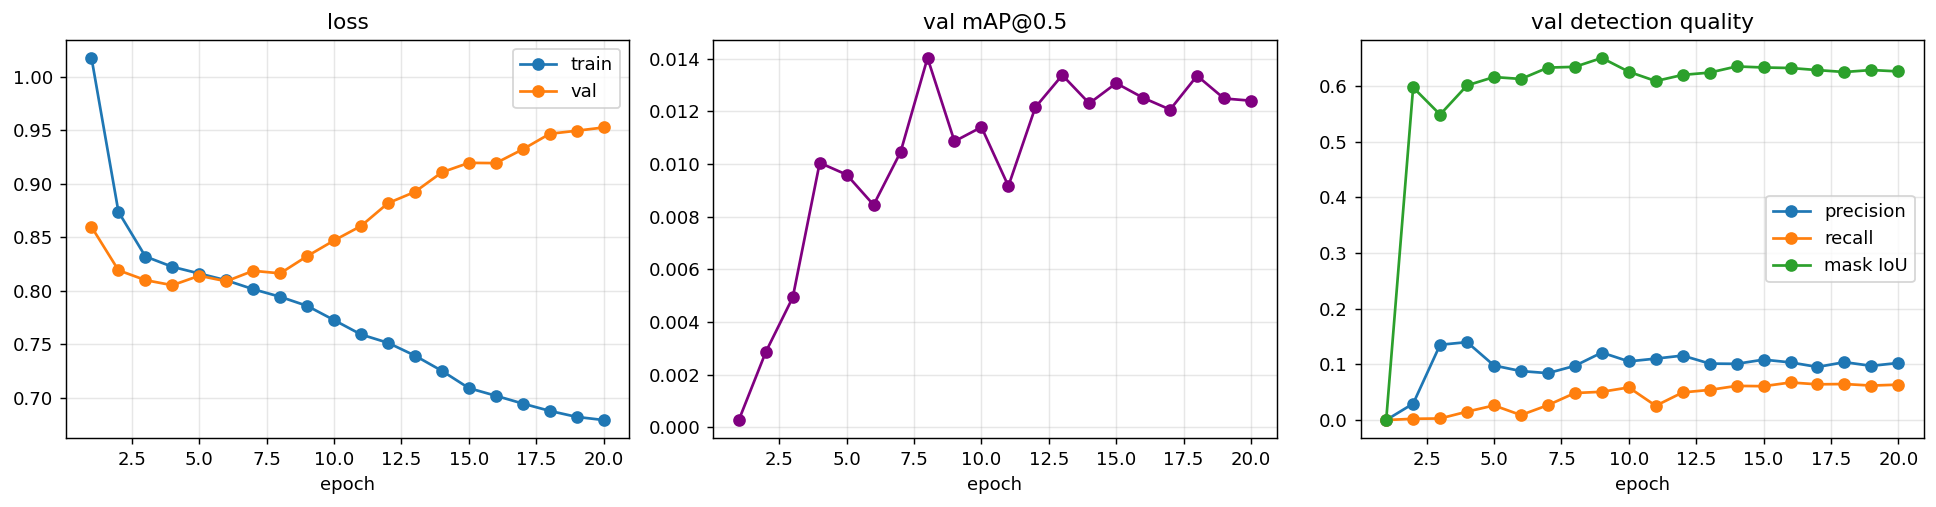
\includegraphics[width=\textwidth]{figures/training_curves.png}
\caption{Training history over $20$ epochs. \emph{Left:} train vs.\ validation
loss --- validation loss turns upward after $\sim\!4$ epochs, indicating
overfitting. \emph{Centre:} validation mAP@0.5, peaking near epoch~$8$.
\emph{Right:} detection quality --- mask IoU saturates early and high, while
precision and recall stay low. The decoupling of mask quality from detection
quality is the central result of this experiment.}
\label{fig:curves}
\end{figure*}

\begin{figure*}[p]
\centering
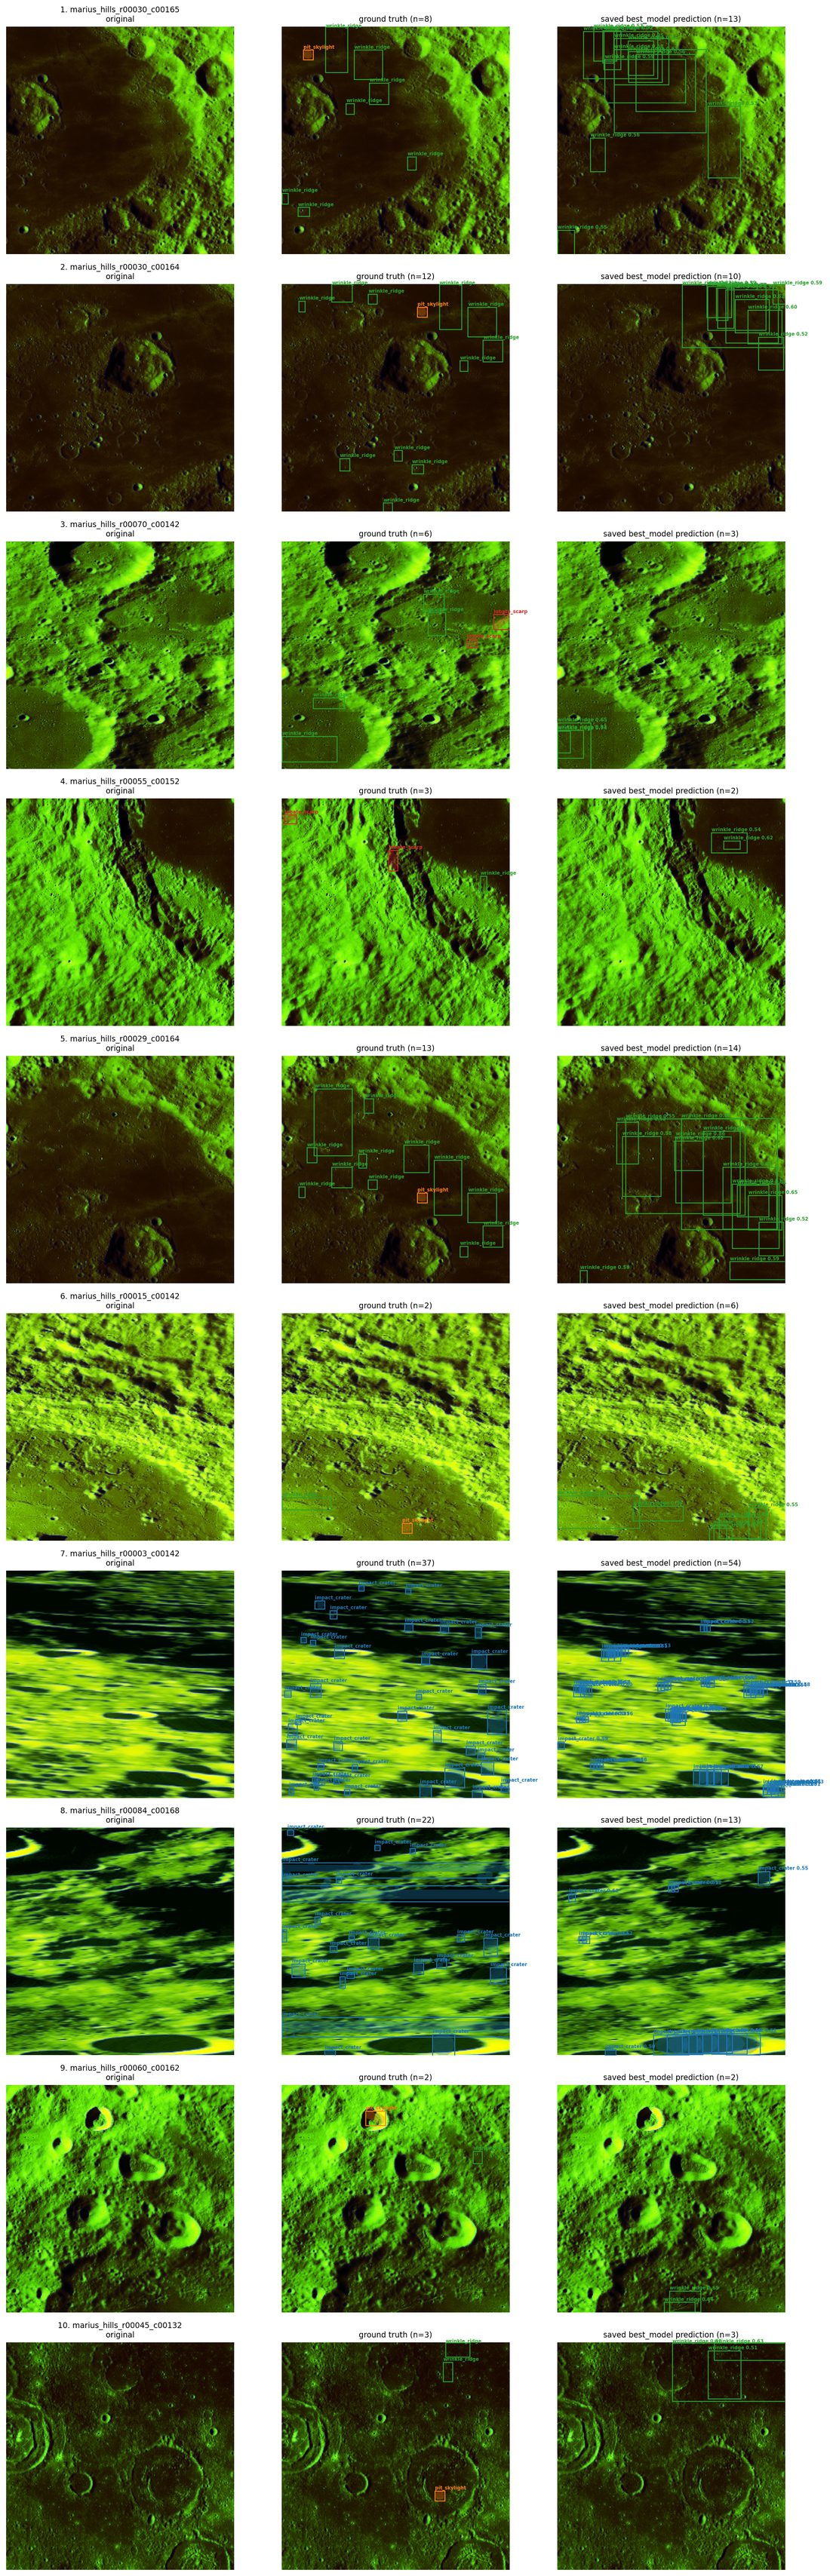
\includegraphics[height=0.92\textheight,keepaspectratio]{figures/prediction_samples.jpg}
\caption{Qualitative results on ten validation tiles from the Marius Hills region.
For each tile: original image (left), ground-truth instances (centre), and
model predictions with class and confidence (right). The network localises and
outlines the larger, higher-contrast craters and ridges reasonably well, but
misses faint or small features and is unreliable on the rare pit/skylight and
lobate-scarp classes.}
\label{fig:qual}
\end{figure*}

\section{SmallUNet: architecture details, losses, and full ablation results}
\label{app:unet}

\subsection{Architecture}

The spatial flow of the network with base width $w=32$ and $256\times 256$ input is:

\[
\begin{array}{c}
(3,\,256,256)
\xrightarrow{\text{inc}}   (32,\,256,256)\\[2pt]
\xrightarrow{\text{down}_1}(64,\,128,128)\\[2pt]
\xrightarrow{\text{down}_2}(128,\,64,64)\\[2pt]
\xrightarrow{\text{down}_3}(256,\,32,32)\\[4pt]
\xrightarrow{\text{up}_1}  (128,\,64,64)\\[2pt]
\xrightarrow{\text{up}_2}  (64,\,128,128)\\[2pt]
\xrightarrow{\text{up}_3}  (32,\,256,256)\\[2pt]
\xrightarrow{\text{out}}   (7,\,256,256)
\end{array}
\]

\noindent
Doubling the base width $w$ quadruples the parameter count; Table~\ref{tab:bw_params} summarises the three widths explored in Study~2.

\begin{table}[htbp]
\centering
\caption{Parameter counts for each base width.}
\label{tab:bw_params}
\begin{tabular}{lrr}
\toprule
Base width $w$ & Channel progression & Parameters \\
\midrule
16 & 16--32--64--128  &    505{,}095 \\
32 & 32--64--128--256 & 2{,}014{,}727 \\
64 & 64--128--256--512 & 8{,}047{,}623 \\
\bottomrule
\end{tabular}
\end{table}

\subsection{Loss definitions}

\paragraph{BCEDiceLoss.}
Binary cross-entropy summed with a soft Dice loss, averaged across classes:
\[
\mathcal{L}_{\text{BCEDice}} = \mathcal{L}_{\text{BCE}} + \mathcal{L}_{\text{Dice}},
\]
\[
\mathcal{L}_{\text{Dice}} = 1 - \frac{1}{C}\sum_{c=1}^{C} \frac{2\sum_i p_i^c\, y_i^c + \varepsilon}{\sum_i p_i^c + \sum_i y_i^c + \varepsilon}
\]
where $p_i^c$ is the predicted probability and $y_i^c$ the ground-truth label for pixel $i$ and class $c$, and $\varepsilon=10^{-6}$ ensures numerical stability.

\paragraph{FocalDiceLoss.}
Replaces the BCE term with the binary focal loss~\citep{lin2017focal} to down-weight easy negatives and focus training on hard positives:
\[
\mathcal{L}_{\text{focal}}(p,y) = -\alpha\,y\,(1-p)^\gamma \log p
                                   -(1-\alpha)(1-y)\,p^\gamma \log(1-p)
\]
with $\gamma=2$ and $\alpha=0.25$. The Dice term additionally uses per-class weights $\mathbf{w} = [1.0,\,4.0,\,5.0,\,5.0,\,5.0,\,5.0,\,5.0]$ to penalise misdetection of rare classes more heavily:
\[
\mathcal{L}_{\text{FocalDice}} = \mathcal{L}_{\text{focal}} + \sum_{c=1}^{C} w_c \,\mathcal{L}_{\text{Dice}}^c
\]

\subsection{Full ablation tables and validation curves}

Tables~\ref{tab:arch_comparison}--\ref{tab:aug_comparison} report the complete per-study results summarised in Sect.~\ref{sec:mr_augmentation}; Figs.~\ref{fig:arch_metrics}--\ref{fig:aug_metrics} show the corresponding per-class validation curves.

\begin{table}[htbp]
\centering
\caption{Architecture ablation on the full dataset (Tesla T4, 30 epochs). Metrics are macro-averaged across the seven classes; Ridge AP is the single-class AP of \texttt{wrinkle\_ridge}.}
\label{tab:arch_comparison}
\resizebox{\columnwidth}{!}{%
\begin{tabular}{lrrrrrrr}
\toprule
Config & Params & Epoch (s) & Final loss & Mean F1 & Mean IoU & Mean AP & Ridge AP \\
\midrule
BCEDice    & 1{,}927{,}207 & 208 & 0.876 & 0.1998 & 0.1666 & 0.1989 & 0.440 \\
FocalDice  & 1{,}927{,}207 & 214 & 3.893 & 0.1994 & 0.1632 & 0.1945 & 0.417 \\
+residual  & 2{,}014{,}727 & 257 & 3.873 & 0.2065 & 0.1675 & 0.1995 & 0.443 \\
+dropout   & 1{,}927{,}207 & 215 & 3.894 & 0.2018 & 0.1643 & 0.1938 & 0.405 \\
\textbf{+both} & \textbf{2{,}014{,}727} & 258 & \textbf{3.863} & \textbf{0.2076} & \textbf{0.1688} & \textbf{0.2004} & \textbf{0.453} \\
\bottomrule
\end{tabular}
}
\end{table}

\begin{table}[htbp]
\centering
\caption{Base-width sweep (FocalDice + residual + dropout=0.3, full T4 run, 30 epochs).}
\label{tab:bw_comparison}
\resizebox{\columnwidth}{!}{%
\begin{tabular}{lrrrrrr}
\toprule
Config & Params & Epoch (s) & Mean F1 & Mean IoU & Mean AP & Ridge AP \\
\midrule
small ($w=16$)   &    505{,}095 &  139 & 0.2031 & 0.1665 & 0.2003 & 0.451 \\
default ($w=32$) & 2{,}014{,}727 &  258 & 0.2093 & 0.1704 & 0.2010 & 0.456 \\
wide ($w=64$)    & 8{,}047{,}623 &  582 & \textbf{0.2153} & \textbf{0.1733} & \textbf{0.2016} & 0.445 \\
\bottomrule
\end{tabular}
}
\end{table}

\begin{table}[htbp]
\centering
\caption{Augmentation study on the random tile split (FocalDice + residual + dropout=0.3, $w=32$, full T4 run, 30 epochs). Crater AP is given for reference; Ridge AP highlights the most affected rare class.}
\label{tab:aug_comparison}
\resizebox{\columnwidth}{!}{%
\begin{tabular}{lrrrrrr}
\toprule
Config & Final loss & Mean F1 & Mean IoU & Mean AP & Crater AP & Ridge AP \\
\midrule
\textbf{no augmentation} & \textbf{3.698} & \textbf{0.2986} & \textbf{0.2289} & \textbf{0.2647} & \textbf{0.947} & \textbf{0.558} \\
+augmentation            &        3.863  &        0.2124  &        0.1724  &        0.2027  &        0.942  &        0.457  \\
\bottomrule
\end{tabular}
}
\end{table}

\begin{figure*}[htbp]
\centering
\begin{subfigure}[b]{0.32\textwidth}
    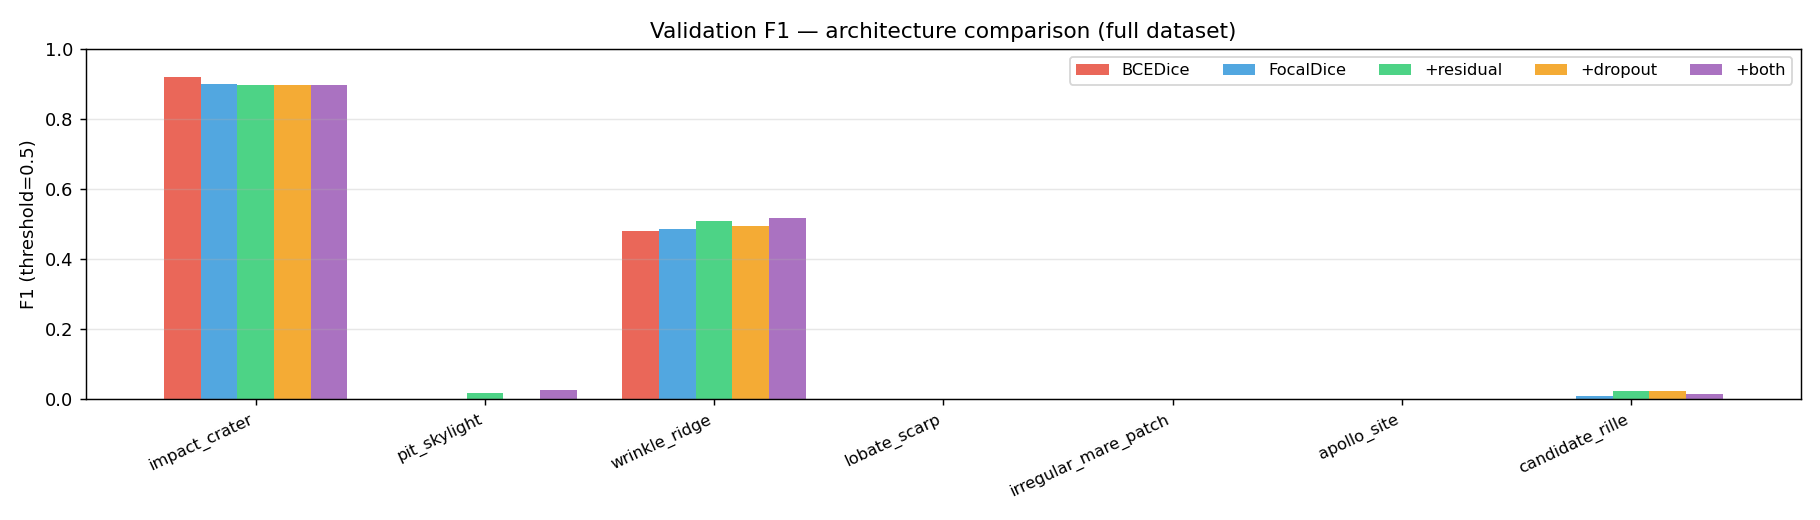
\includegraphics[width=\textwidth]{figures/MR/cloudveneto_arch_val_f1.png}
    \caption{Validation F1}
\end{subfigure}
\hfill
\begin{subfigure}[b]{0.32\textwidth}
    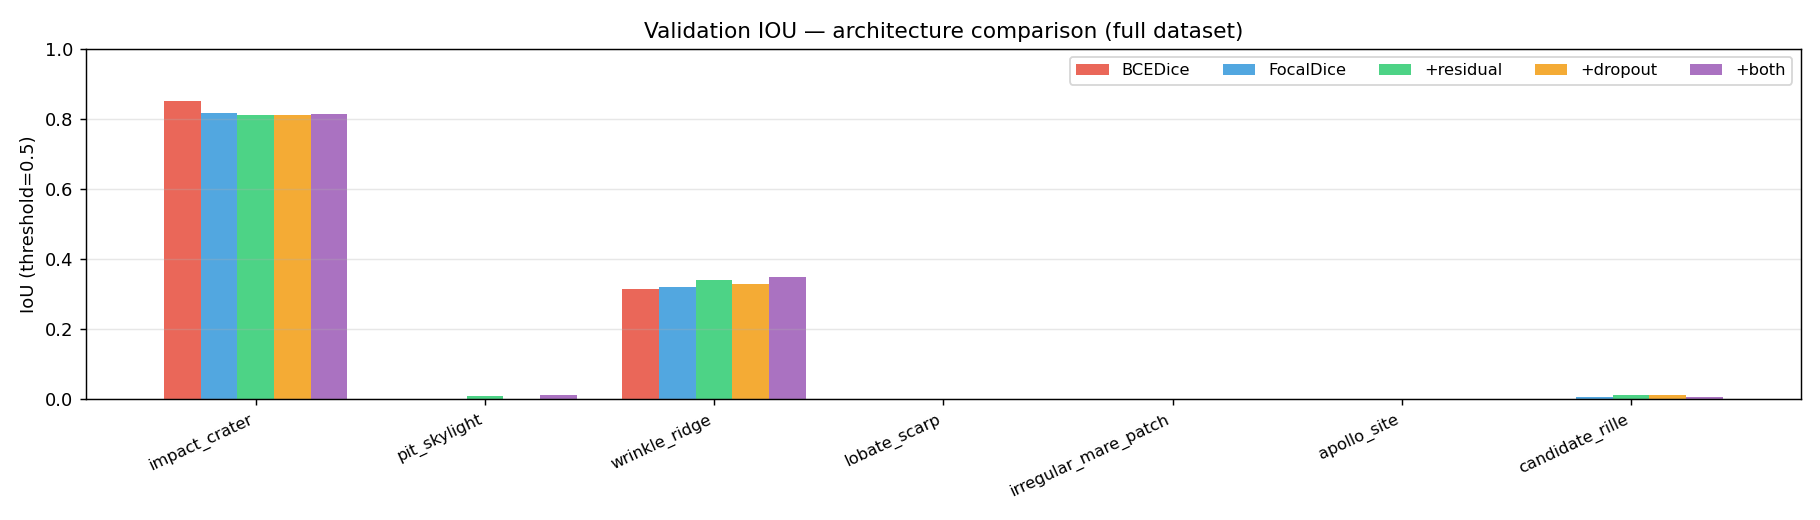
\includegraphics[width=\textwidth]{figures/MR/cloudveneto_arch_val_iou.png}
    \caption{Validation IoU}
\end{subfigure}
\hfill
\begin{subfigure}[b]{0.32\textwidth}
    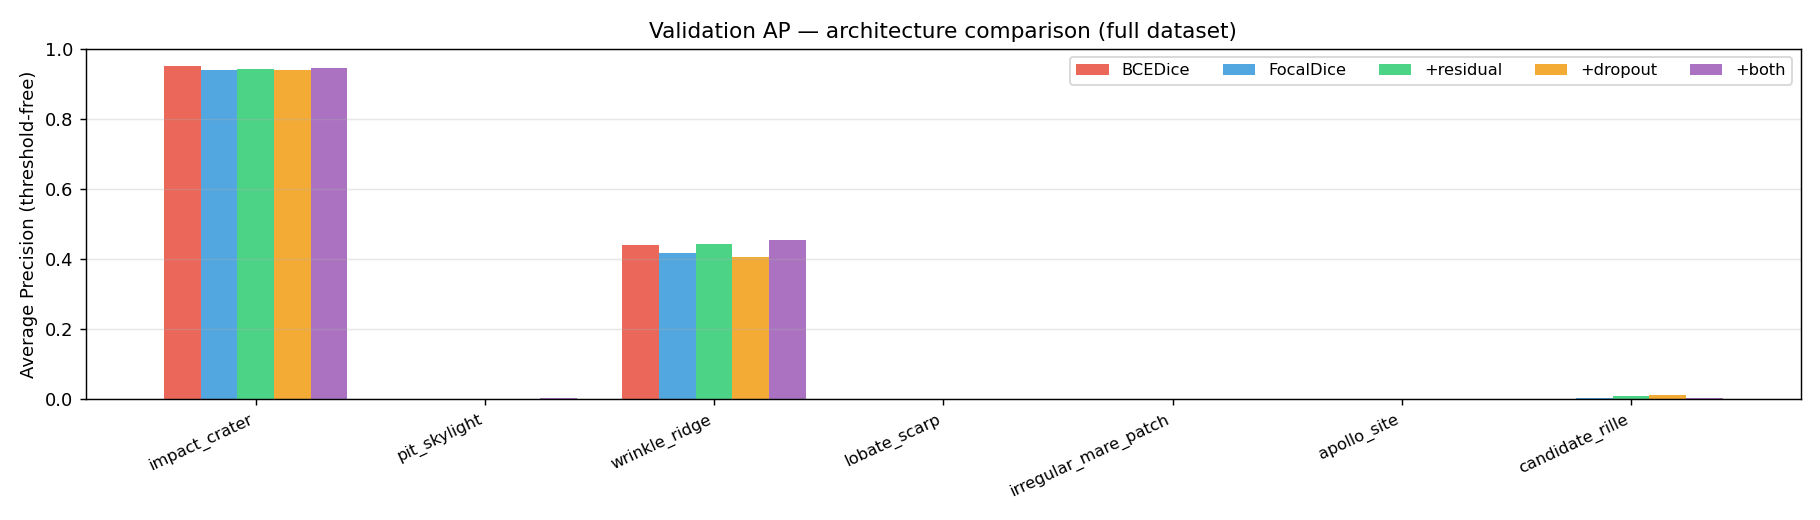
\includegraphics[width=\textwidth]{figures/MR/cloudveneto_arch_val_ap.png}
    \caption{Validation AP}
\end{subfigure}
\caption{Per-class validation metrics across training epochs for the five architecture configurations (full T4 run, 30 epochs). \textbf{+both} (residual + dropout + FocalDice) achieves the highest aggregate performance on all three metrics.}
\label{fig:arch_metrics}
\end{figure*}

\begin{figure*}[htbp]
\centering
\begin{subfigure}[b]{0.32\textwidth}
    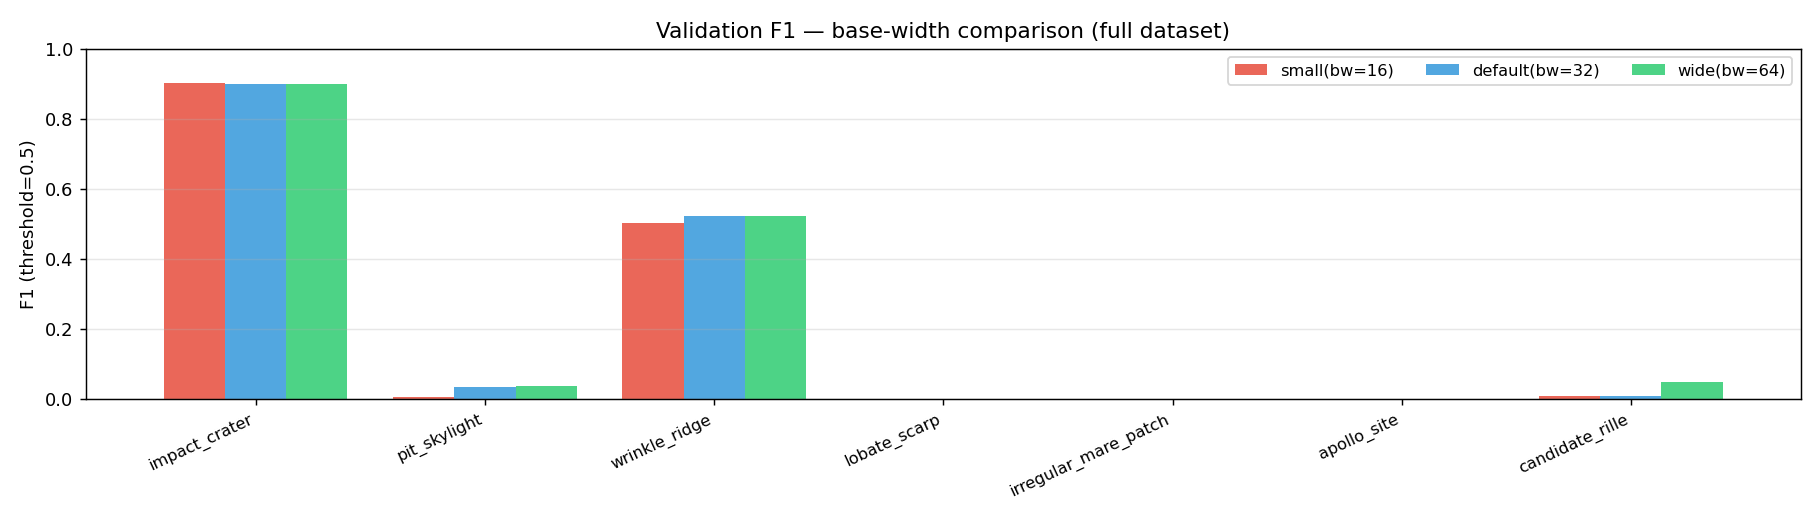
\includegraphics[width=\textwidth]{figures/MR/cloudveneto_bw_val_f1.png}
    \caption{Validation F1}
\end{subfigure}
\hfill
\begin{subfigure}[b]{0.32\textwidth}
    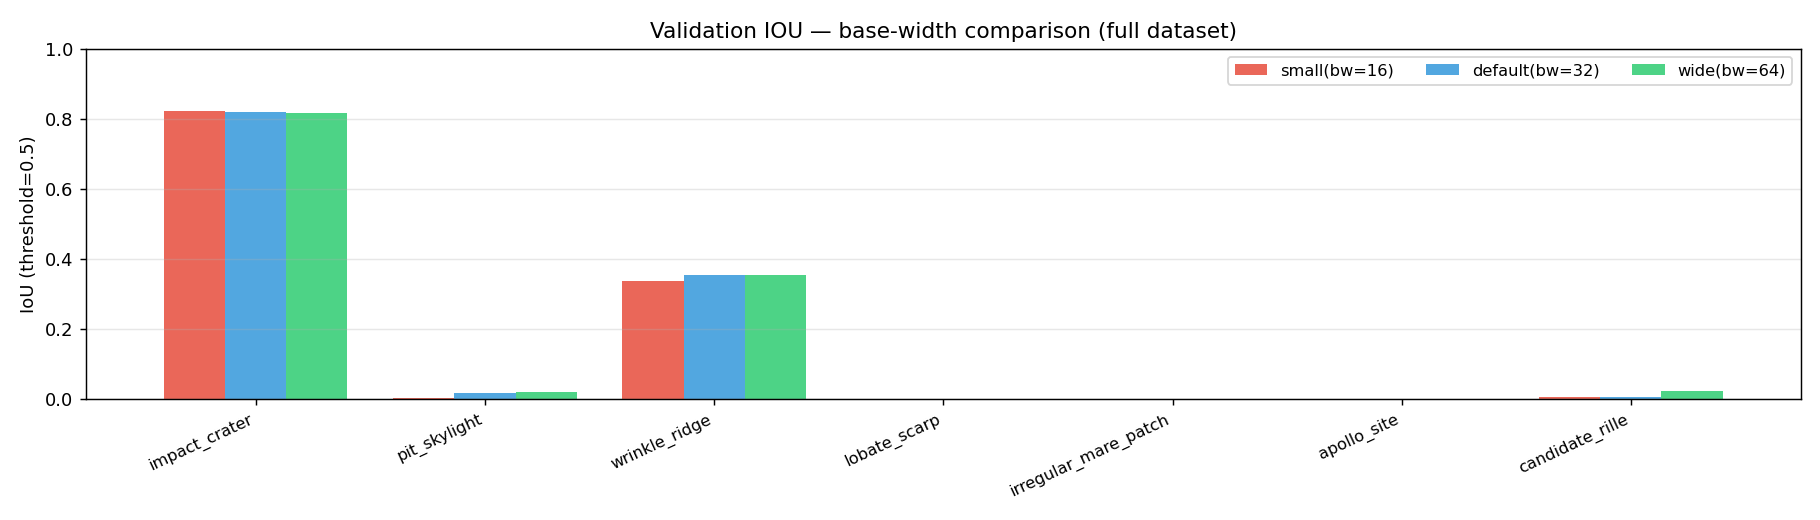
\includegraphics[width=\textwidth]{figures/MR/cloudveneto_bw_val_iou.png}
    \caption{Validation IoU}
\end{subfigure}
\hfill
\begin{subfigure}[b]{0.32\textwidth}
    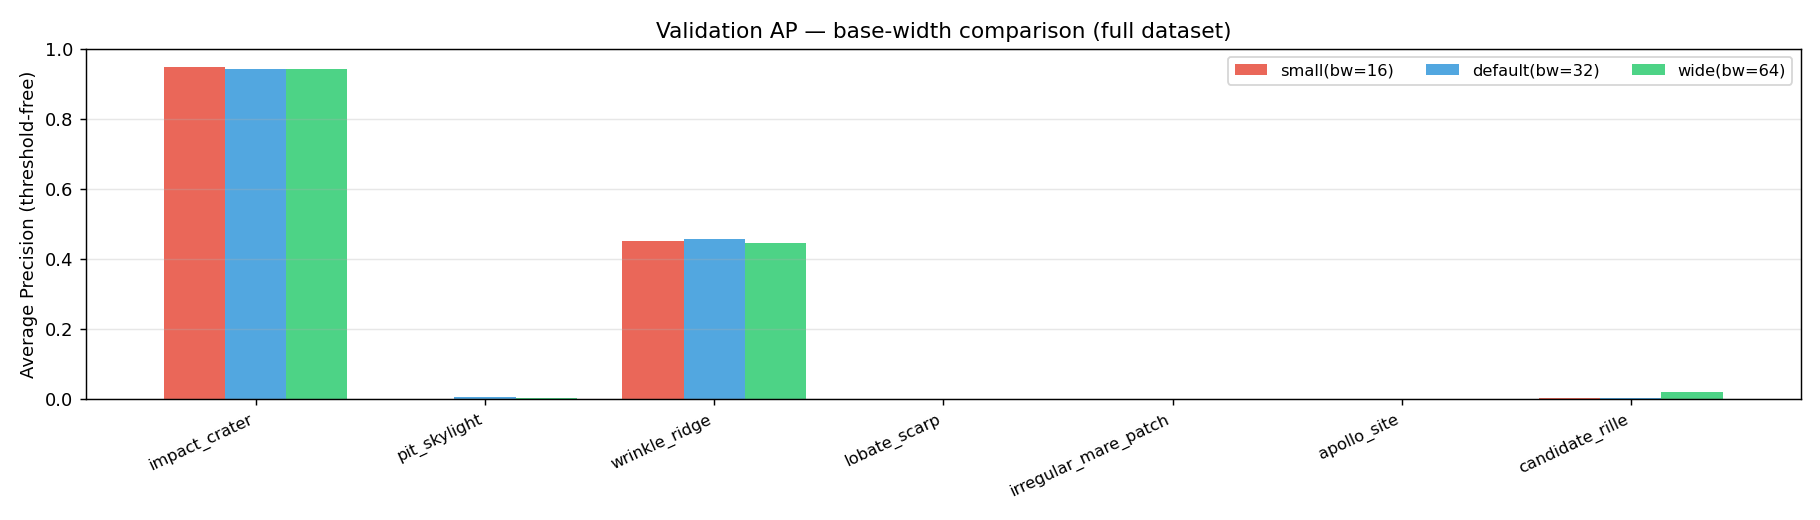
\includegraphics[width=\textwidth]{figures/MR/cloudveneto_bw_val_ap.png}
    \caption{Validation AP}
\end{subfigure}
\caption{Validation metrics for three network widths (full T4 run, 30 epochs). Wider networks achieve marginally higher scores but exhibit severely diminishing returns in parameters and training time.}
\label{fig:bw_metrics}
\end{figure*}

\begin{figure*}[htbp]
\centering
\begin{subfigure}[b]{0.32\textwidth}
    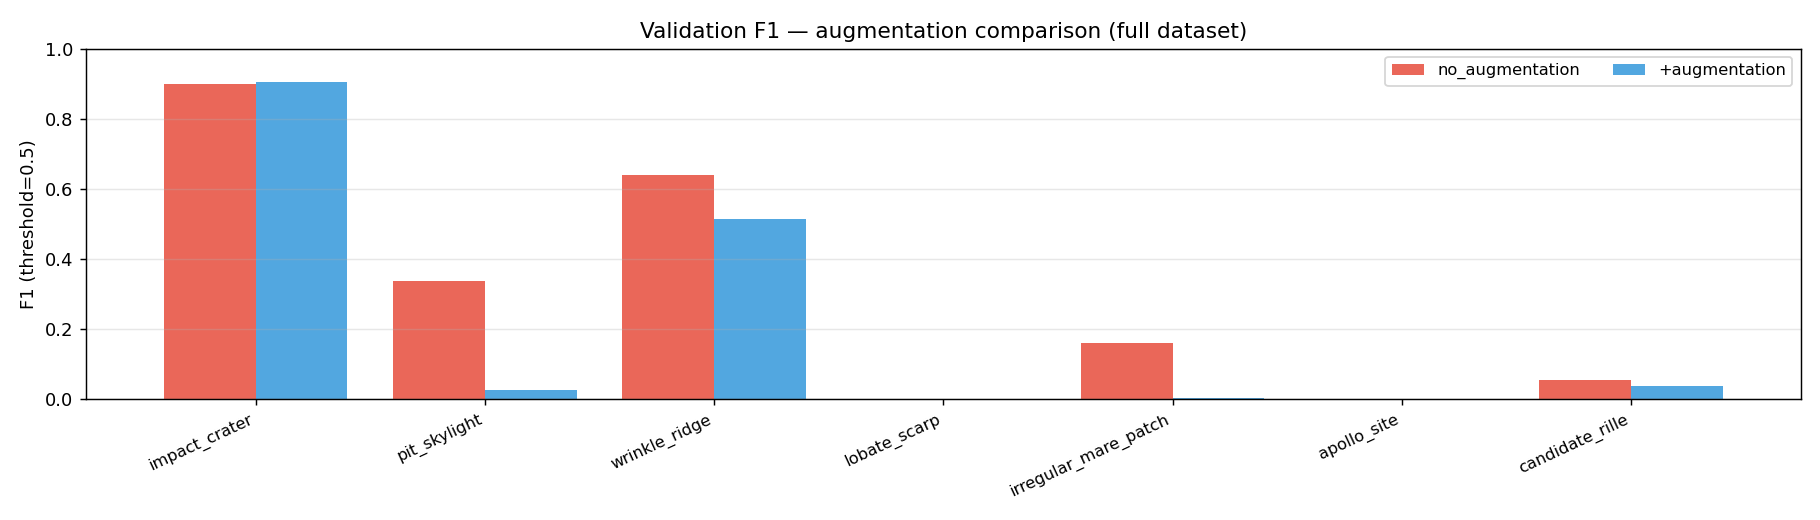
\includegraphics[width=\textwidth]{figures/MR/cloudveneto_aug_val_f1.png}
    \caption{Validation F1}
\end{subfigure}
\hfill
\begin{subfigure}[b]{0.32\textwidth}
    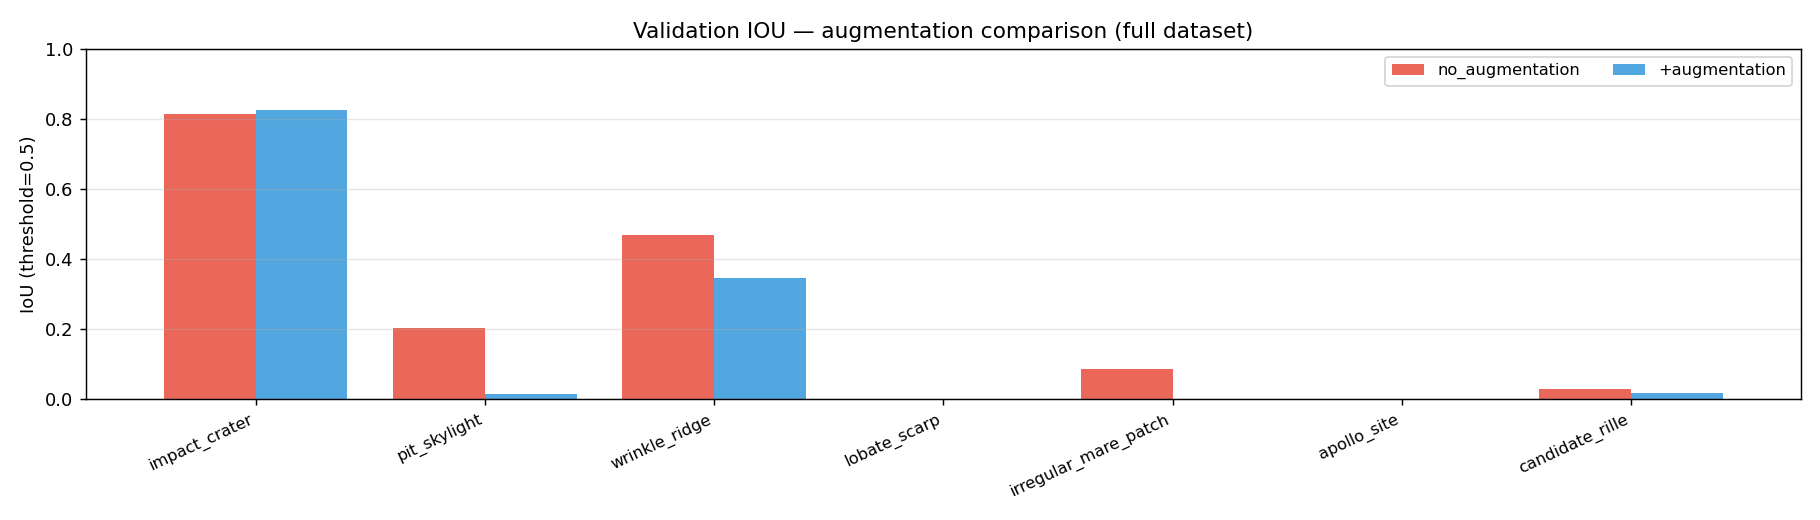
\includegraphics[width=\textwidth]{figures/MR/cloudveneto_aug_val_iou.png}
    \caption{Validation IoU}
\end{subfigure}
\hfill
\begin{subfigure}[b]{0.32\textwidth}
    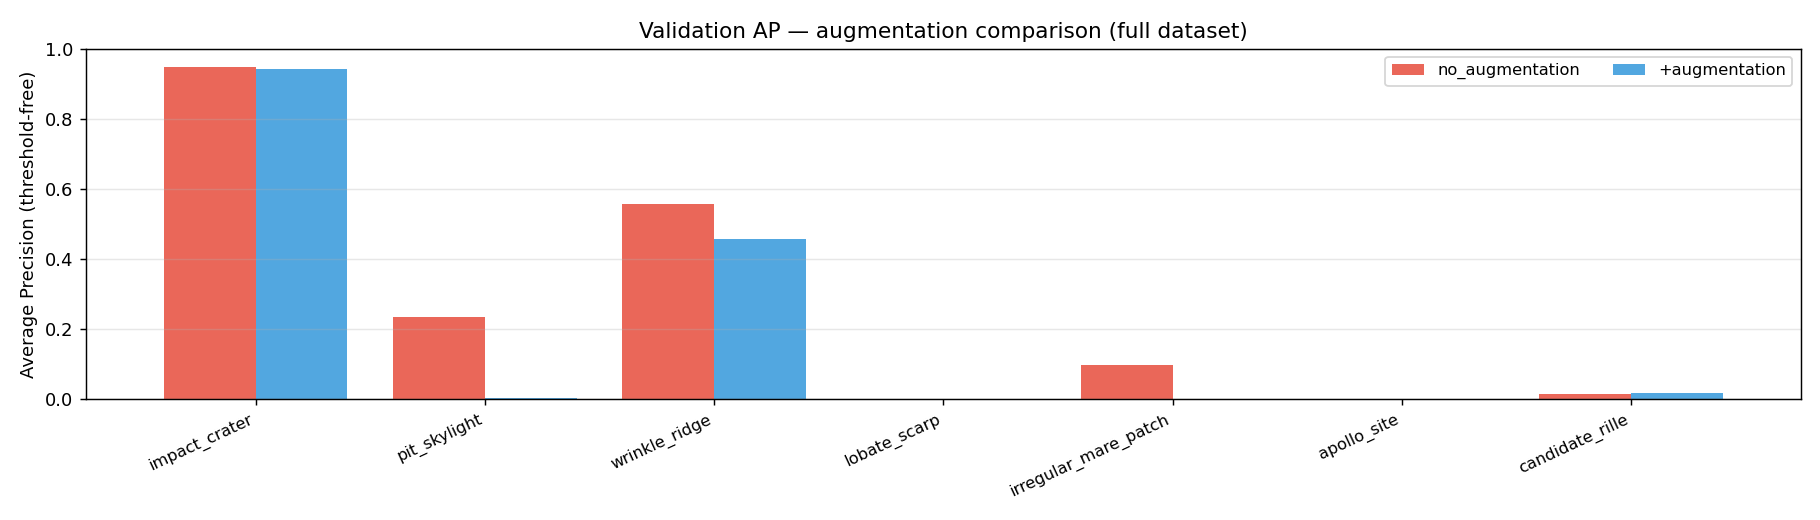
\includegraphics[width=\textwidth]{figures/MR/cloudveneto_aug_val_ap.png}
    \caption{Validation AP}
\end{subfigure}
\caption{Validation metrics with and without geometric augmentation (random tile split, full T4 run, 30 epochs). No augmentation outperforms the augmented training on all metrics.}
\label{fig:aug_metrics}
\end{figure*}

\section{YOLOv8: label statistics and training diagnostics}
\label{app:yolo}

Tables~\ref{tab:class_dist} and~\ref{tab:class_dist_reduced} report the box-level class distributions of the two training datasets of Sect.~\ref{sec:yolo}; Figs.~\ref{fig:class_dist}--\ref{fig:metrics_comparison} collect the label statistics and training diagnostics.

\begin{table}[htbp]
\centering
\caption{Per-class instance distribution in the full lunar surface feature dataset.}
\label{tab:class_dist}
\resizebox{\columnwidth}{!}{%
\begin{tabular}{llrr}
\hline
\textbf{Class ID} & \textbf{Class Label} & \textbf{Instances} & \textbf{Proportion (\%)} \\
\hline
class0 & Impact Crater         & 382,122 & 95.51 \\
class2 & Wrinkle Ridge         &  16,133 &  4.03 \\
class3 & Lobate Scarp          &     674 &  0.17 \\
class1 & Pit Skylight          &     328 &  0.08 \\
class4 & Irregular Mare Patch  &     191 &  0.05 \\
class5 & Apollo Site           &     161 &  0.04 \\
class6 & Candidate Rille       &      82 &  0.02 \\
\hline
\textbf{Total} & & \textbf{399,691} & \textbf{100.00} \\
\hline
\end{tabular}
}
\end{table}

\begin{table}[htbp]
\centering
\caption{Per-class instance distribution of the reduced dataset after excluding the impact crater class.}
\label{tab:class_dist_reduced}
\resizebox{\columnwidth}{!}{%
\begin{tabular}{llrr}
\hline
\textbf{Class ID} & \textbf{Class Label} & \textbf{Instances} & \textbf{Proportion (\%)} \\
\hline
class1 & Wrinkle Ridge        & 16,115 & 92.59 \\
class2 & Lobate Scarp         &    664 &  3.81 \\
class0 & Pit Skylight         &    311 &  1.79 \\
class4 & Apollo Site          &    156 &  0.90 \\
class3 & Irregular Mare Patch &    148 &  0.85 \\
class5 & Candidate Rille      &     92 &  0.53 \\
\hline
\textbf{Total} & & \textbf{17,486} & \textbf{100.00} \\
\hline
\end{tabular}
}
\end{table}

\begin{figure}[htbp!]
    \centering
    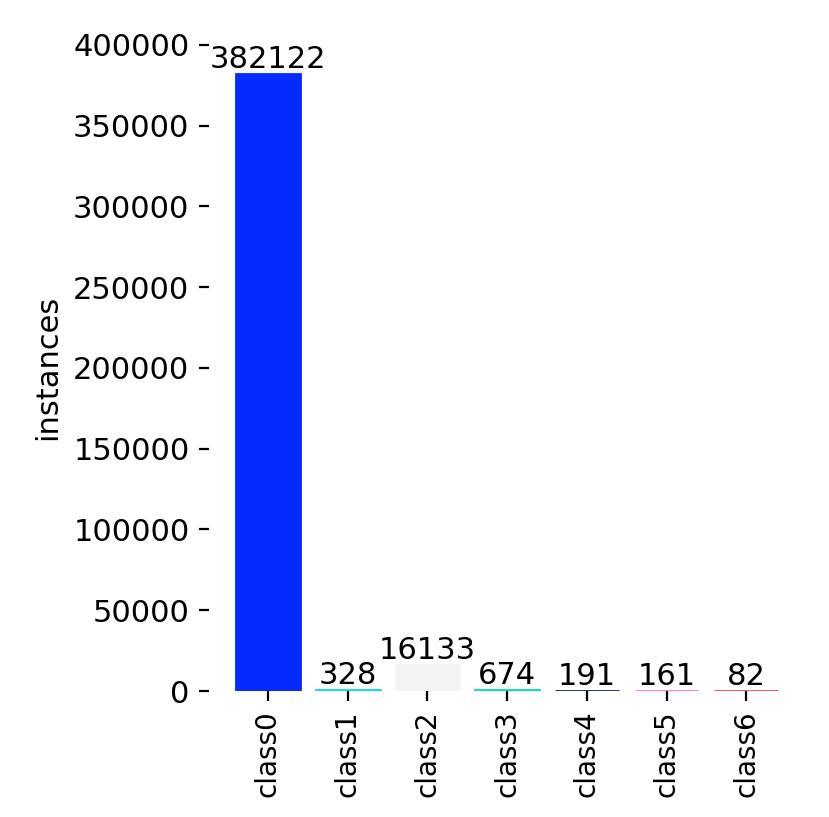
\includegraphics[width=0.85\linewidth]{./imageswithzero/labels_copy.jpg}
    \caption{Class instance distribution of the full dataset across
    seven categories. The impact crater class (class0) dominates with 382,122 instances,
    representing 95.51\% of all annotations.}
    \label{fig:class_dist}
\end{figure}

\begin{figure}[htbp!]
    \centering
    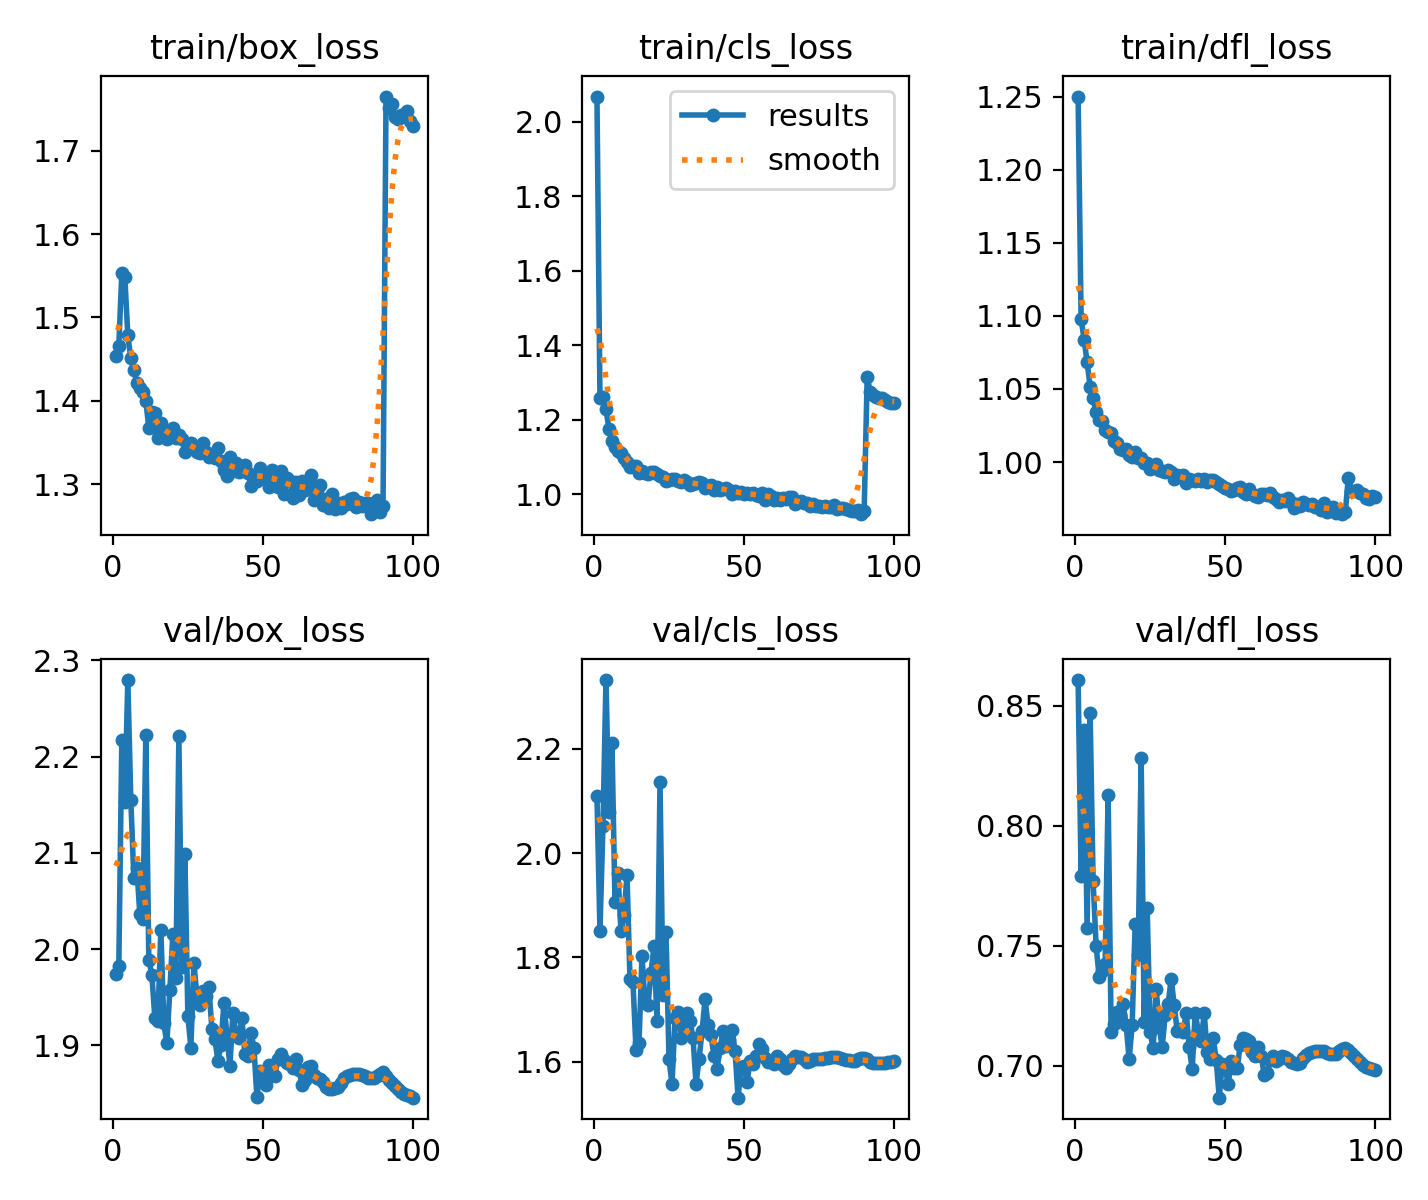
\includegraphics[width=0.95\linewidth]{./imageswithzero/loss.png}
    \caption{Training and validation loss curves over 100 epochs for the YOLOv8n
    model trained on the full seven-class dataset, including bounding box loss (box\_loss),
    classification loss (cls\_loss), and distribution focal loss (dfl\_loss).}
    \label{fig:loss_curves}
\end{figure}

\begin{figure}[htbp!]
    \centering
    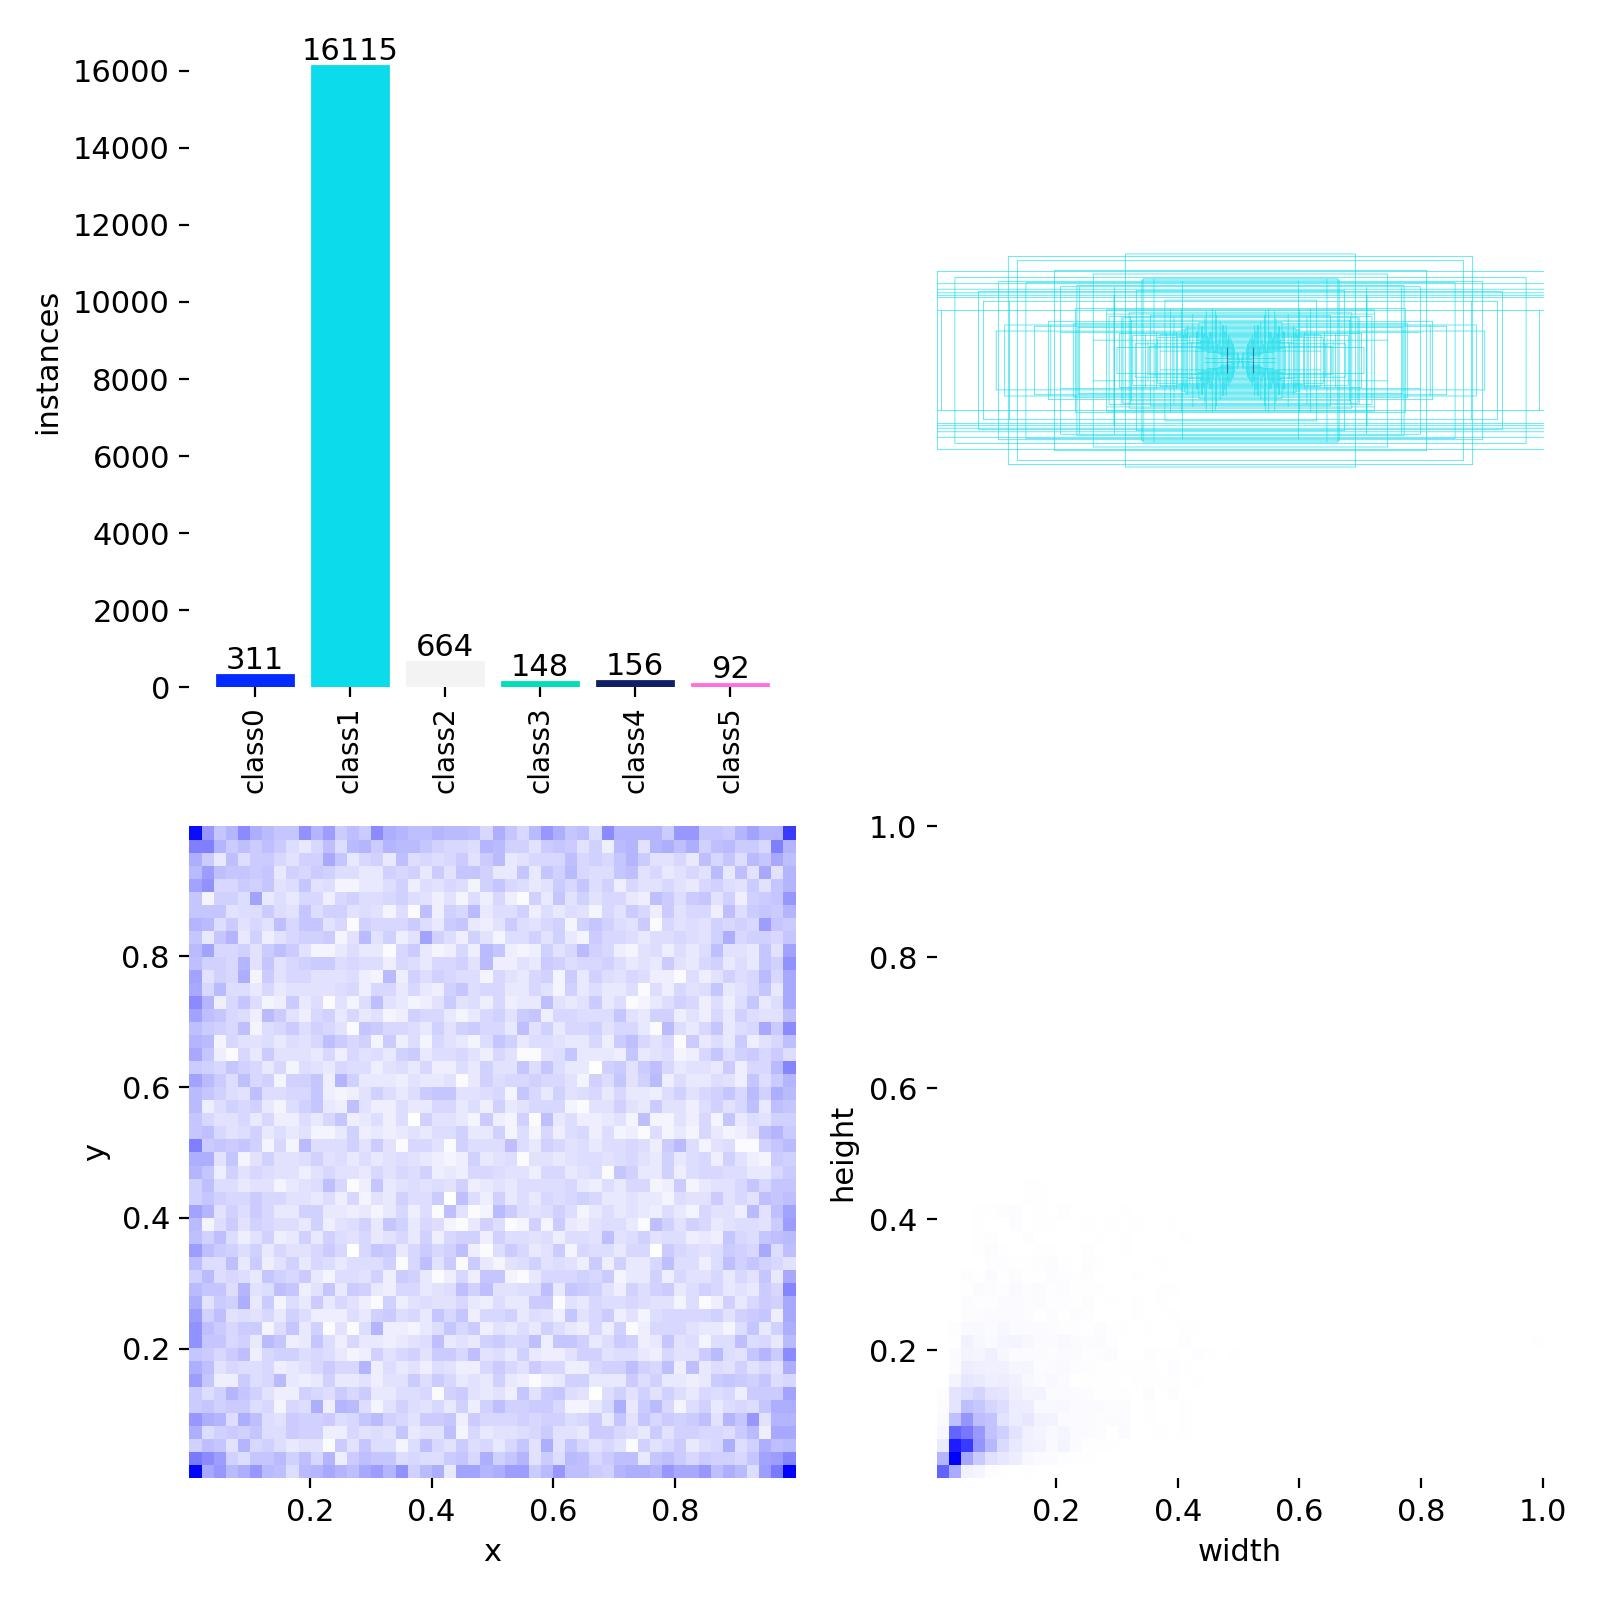
\includegraphics[width=0.85\linewidth]{imageswithoutzero/labels(1).jpg}
    \caption{Class instance distribution and spatial statistics of the reduced
    dataset after removing the impact crater class. The spatial heatmap shows a
    more uniform distribution of object centers across the image plane, while
    bounding boxes remain concentrated at small width-height values ($<$0.2),
    confirming the small-scale nature of the detected features.}
    \label{fig:labels_reduced}
\end{figure}

\begin{figure}[htbp!]
    \centering
    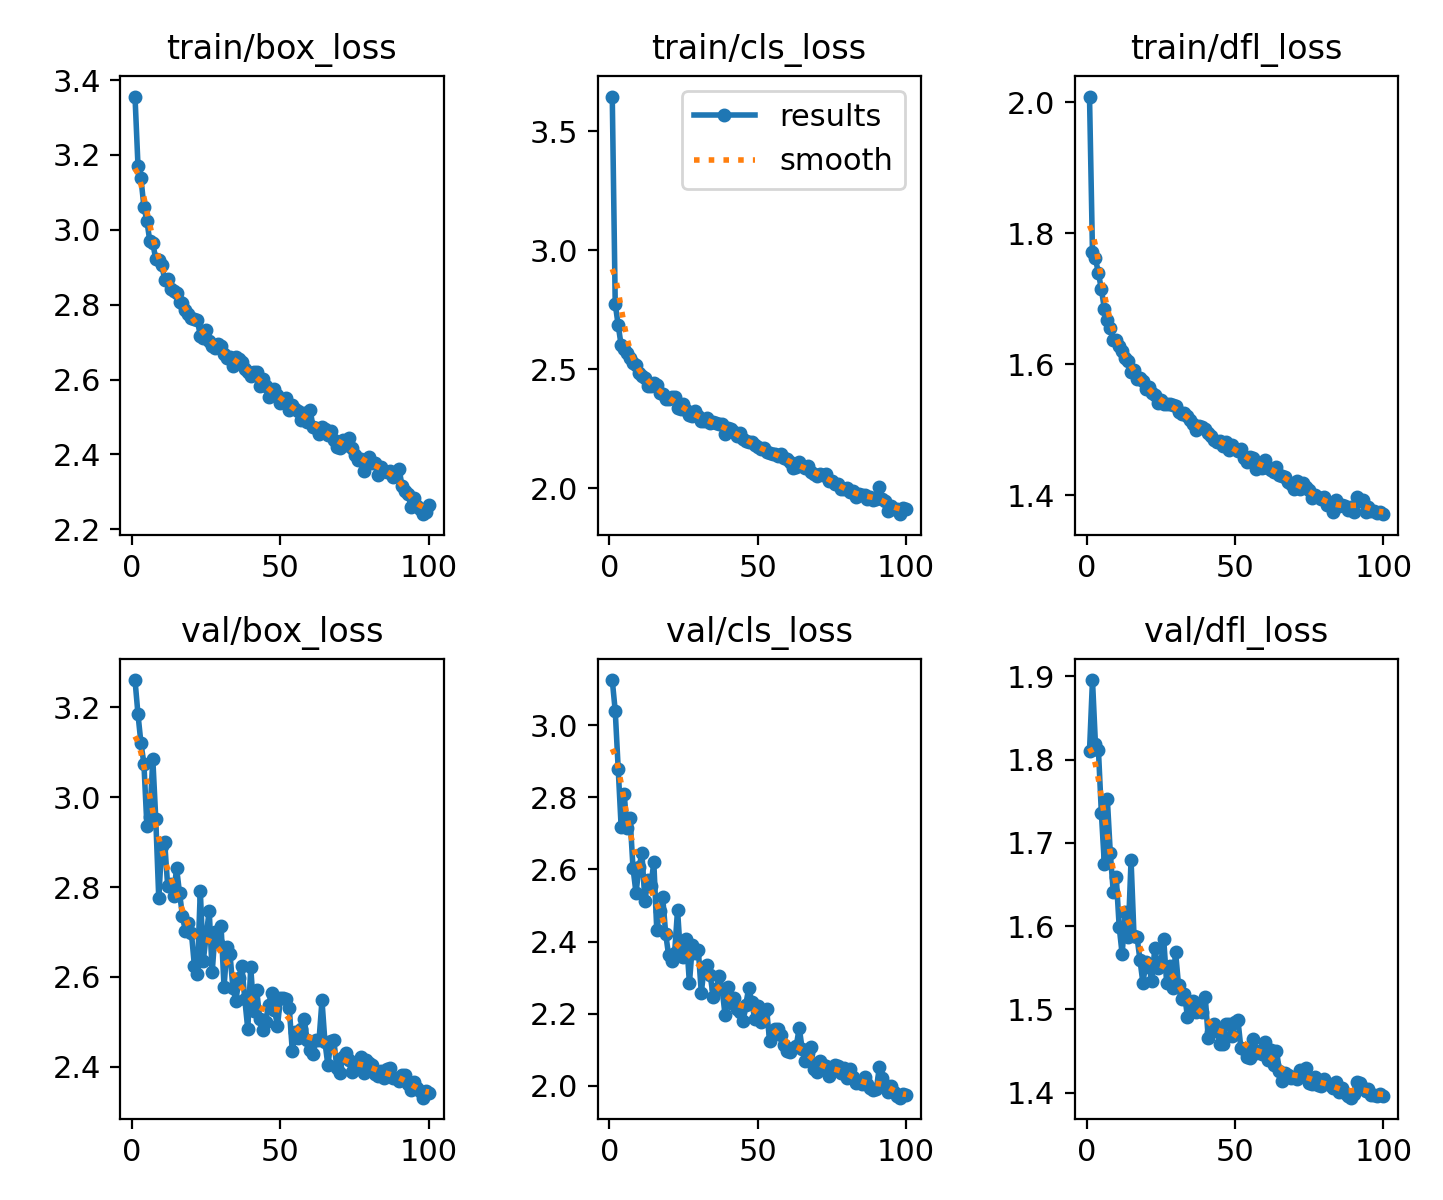
\includegraphics[width=0.95\linewidth]{imageswithoutzero/results(1)copy.png}
    \caption{Training and validation loss curves over 100 epochs for the YOLOv8n
    model trained on the reduced dataset (impact crater class excluded), showing
    box loss, classification loss, and distribution focal loss (DFL).}
    \label{fig:loss_reduced}
\end{figure}

\begin{figure}[htbp!]
    \centering
    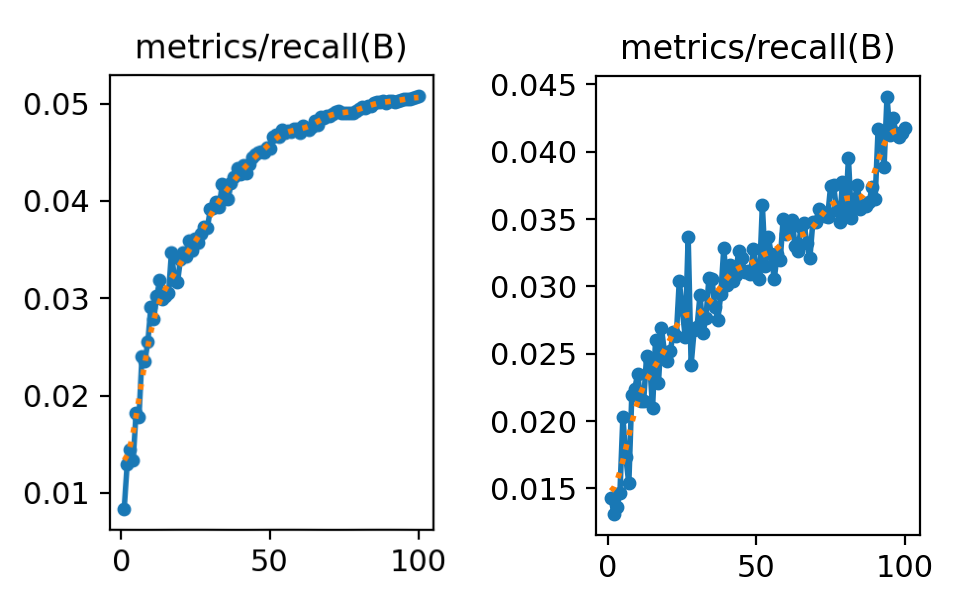
\includegraphics[width=\linewidth]{./image.png}
    \caption{Recall curves over 100 training epochs for both
    experiments. Right: full dataset --- recall grows slowly to $\sim$0.05,
    reflecting the dominance of the impact crater class. Left: reduced
    dataset --- recall grows steadily to $\sim$0.043, now spread across the
    six rare classes rather than concentrated on craters.}
    \label{fig:metrics_comparison}
\end{figure}

\section{South pole: inference diagnostics}
\label{app:southpole}

Figure~\ref{fig:south_pole_diag} shows the per-class confidence diagnostics behind Table~\ref{tab:south_pole_stats}.

\begin{figure*}[htbp]
\centering
\begin{subfigure}[b]{0.48\textwidth}
    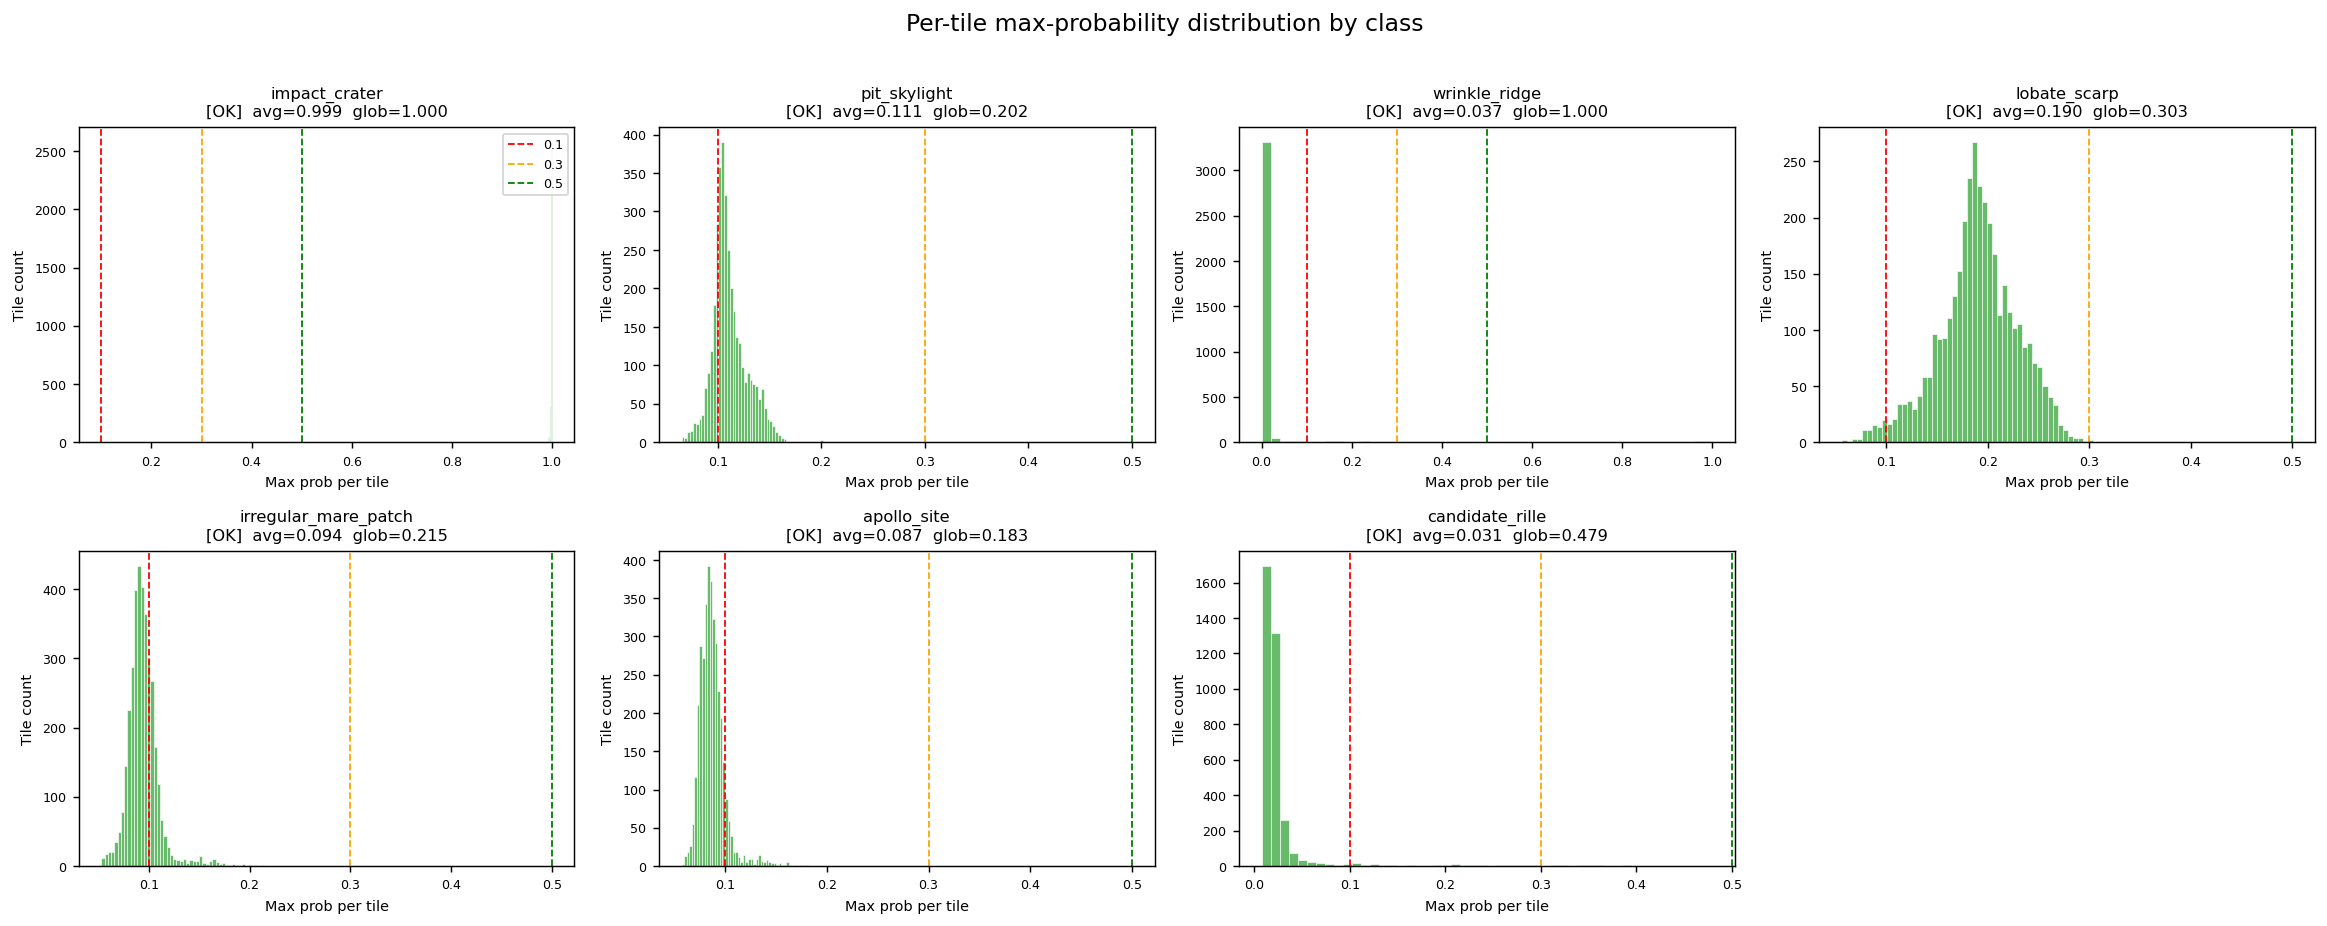
\includegraphics[width=\textwidth]{figures/MR/diagnostics_distributions.png}
    \caption{Per-tile max-probability distributions.}
\end{subfigure}
\hfill
\begin{subfigure}[b]{0.48\textwidth}
    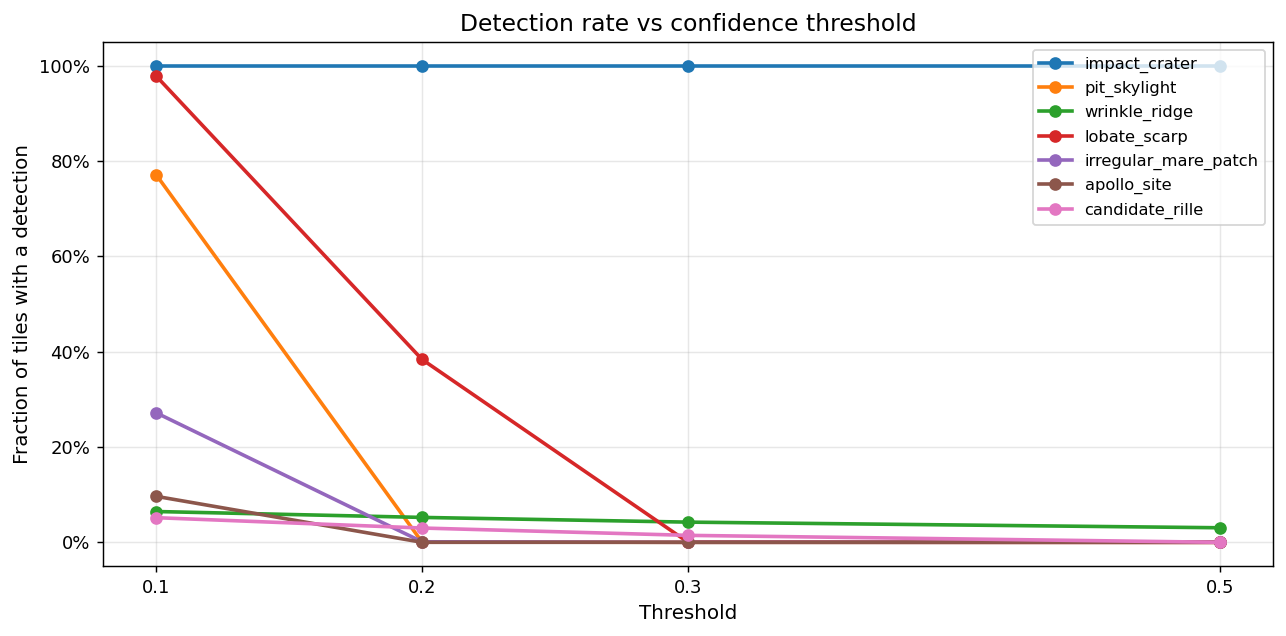
\includegraphics[width=\textwidth]{figures/MR/diagnostics_detection_rates.png}
    \caption{Detection rate vs.\ confidence threshold.}
\end{subfigure}
\caption{South pole inference diagnostics across 3\,639 tiles. Impact craters are detected with near-certainty across the entire region. All other classes exhibit strongly right-skewed distributions with low average confidence, reflecting both the domain shift from Marius Hills and the scarcity of these features at the south pole.}
\label{fig:south_pole_diag}
\end{figure*}

\end{appendix}




\end{document}
